\chapter{Analiza i modelowanie}
W rozdziale tym opisane jest wykonane przez nas modelowanie. Wspieramy się tutaj wybranymi fragmentami kodu, natomiast cały kod dostępny jest w oddzielnym pliku.

\section{Wstępne przygotowanie zbioru danych} 
W pierwszym etapie, nazwijmy wstępnym do tworzenia modeli, stworzyłyśmy notatnik w Google Colab zintegrowany z Dykiem Google i wczytałyśmy dane do \verb|DataFrame|'a.

\begin{lstlisting}[language=Python,frame=single, breaklines=true,caption=Wczytywanie surowych danych z Dysku Google do pandas.DataFrame'a.,label=code:readData]
import pandas as pd
from google.colab import drive
drive.mount('/content/drive')

data_file = "drive/MyDrive/IMDB_Dataset.csv"
data = pd.read_csv(data_file, header=0, low_memory=False)
\end{lstlisting}

\noindent Surowe dane przedstawione są na poniższym rysunku (Rysunek. \ref{fig:rawDataset}). \\ \\
\noindent Jak widać zbiór danych składa się z dwóch interesujących nas kolumn. Kolumna pierwsza o nazwie \textit{review} (dtype: object) zawiera surowe treści recenzji filmów wraz z tagami w języku HTML, natomiast kolumna druga o nazwie \textit{sentiment} zawiera informację, czy dana recenzja uznawana jest jako pozytywna czy negatywna --- etykieta (dtype: object). \\

%%%  ------------> obrazek
\begin{figure}[H]
	\centering
	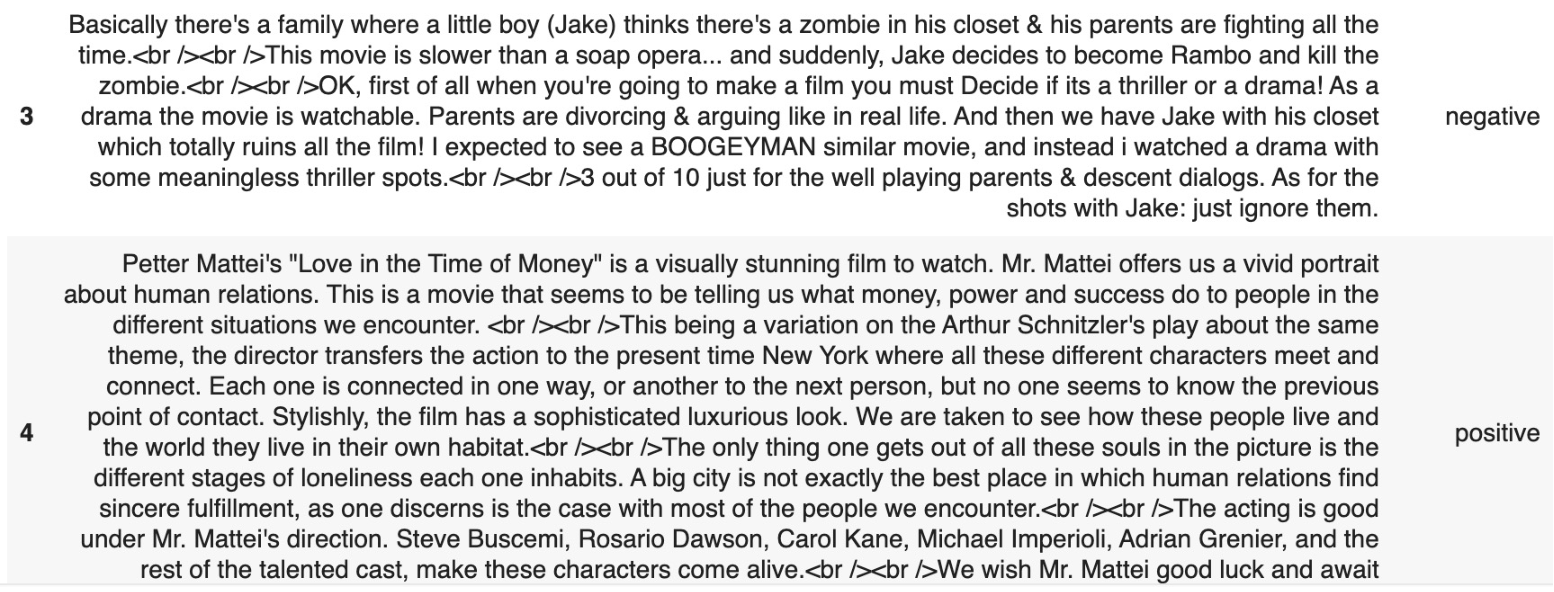
\includegraphics[width=0.95\linewidth]{images/chapter3/raw-data-example.pdf}
	\caption{Przykładowe próbki z surowego zbioru danych recenzji filmowych IMDB.}
	\label{fig:rawDataset}
\end{figure}


\noindent Jako że model matematyczny działa na wartościach liczbowych, kolumnę etykiet słownych zamieniłyśmy na etykiety w postaci liczb, gdzie etykieta 0 oznacza recenzję negatywną, a etykieta 1 pozytywną (zmiana dtype z object na int64). Na tym etapie usunęłyśmy również tagi HTML wykorzystując pakiet \verb|bs4|.


\begin{lstlisting}[language=Python,frame=single, breaklines=true, caption=Zmiana etykiet z typu obiekt na typ liczbowy.,label=code:labelChange]
labels = labels.replace("negative", 0)
labels = labels.replace("positive", 1)

from bs4 import BeautifulSoup
reviews = reviews.apply(lambda text: BeautifulSoup(text).get_text())
reviews.head()
\end{lstlisting}

%%%  ------------> obrazek
\begin{figure}[H]
	\centering
	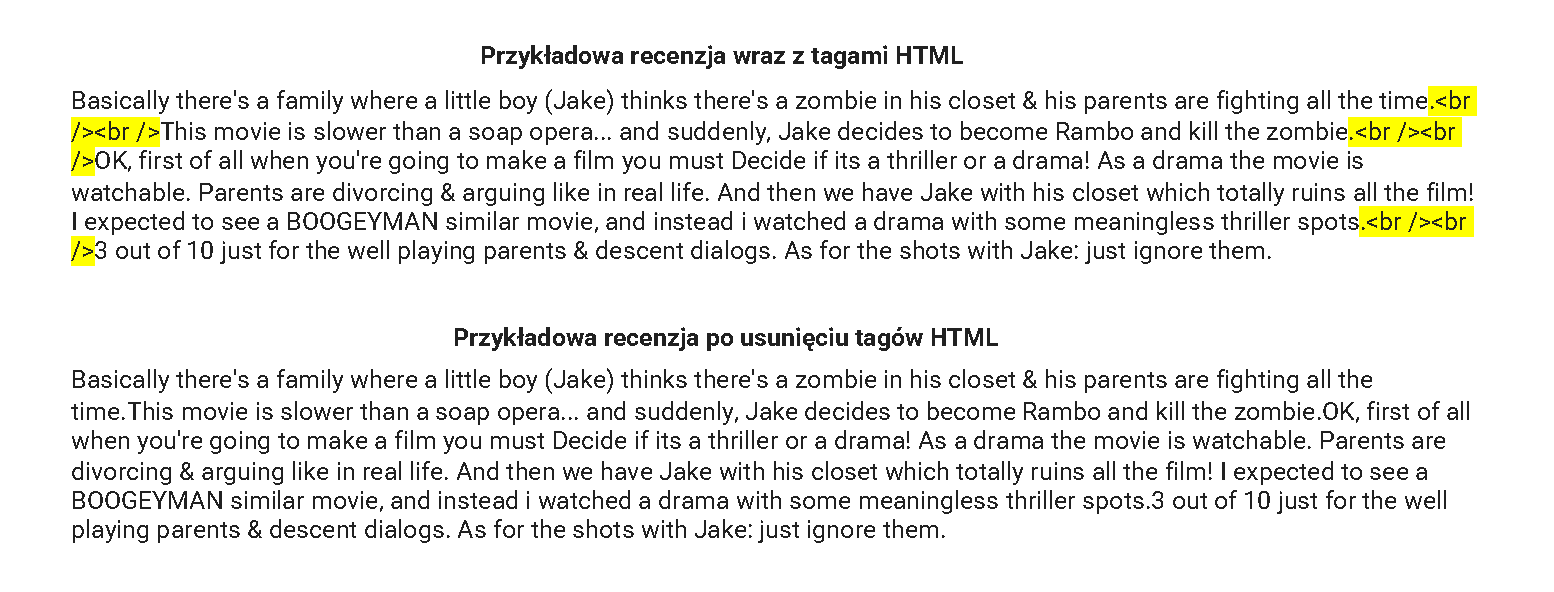
\includegraphics[width=0.95\linewidth]{images/chapter3/cleaned-data-example.pdf}
	\caption{Przykładowa recenzja przed usunięciem tagów HTML (surowa) oraz po usunięciu tagów.}
	\label{fig:cleaned}
\end{figure}

\noindent Przy okazji sprawdziłyśmy, czy zbiór jest dobrze zbalansowany --- czy liczba recenzji pozytywnych i negatywnych jest porównywalna. W kolejnym etapie podzieliłyśmy zbiór danych na dane treningowe i testowe w proporcji 80:20 używając metody \verb|train_test_split| z biblioteki \verb|Pandas| i ponownie sprawdziłyśmy, czy po wykonanym podziale nasze podzbiory są zbalansowane (train: 20 044 recenzje pozytywne i 19 956 recenzji negatywnych oraz test: 4 956 recenzji pozytywnych i 5 044 recenzje negatywne).

\begin{lstlisting}[language=Python,frame=single, breaklines=true, caption=Podział danych na zbiór treningowy i testowy.,label=code:split]
from sklearn.model_selection import train_test_split
train_data, test_data, train_labels, test_labels = train_test_split(reviews, labels, test_size=0.2, random_state=1)

train_labels = train_labels.astype('int')
test_labels = test_labels.astype('int')
\end{lstlisting}

\noindent Następnie bazując na wbudowanej liście angielskich słów stop-words rozbudowanej o znaki interpunkcyjne i kilka własnych znaków (głównie cudzysłowów), usunęłyśmy wyrazy popularnie występujące a więc i nic nie wnoszące, po czym dokonałyśmy prostej wektoryzacji używając klasy \verb|CountVectorizer|.

\begin{lstlisting}[language=Python,frame=single, breaklines=true, caption=Wektoryzacja zbiorów danych --- treningowego i testowego.,label=code:vectorization]
from sklearn.feature_extraction.text import CountVectorizer
count_vectorizer = CountVectorizer(stop_words=english_stopwords) 
train_data_count = count_vectorizer.fit_transform(train_data)
test_data_count = count_vectorizer.transform(test_data)
\end{lstlisting}



\section{Modelowanie}
Po wstępnym przygotowaniu danych przyszedł czas na modelowanie. Stworzyłyśmy 4 rodzaje modeli oraz dla każdego z nich wykonałyśmy optymalizacje hiperparametrów aby otrzymać jak najlepsze wyniki. W pierwszej kolejności stworzyłyśmy model wykorzystujący układ drzew decyzyjnych --- Las Losowy (\textit{Random Forest}).

\subsection{Las losowy}

Model klasyfikujący stworzyłyśmy używając klasy \verb|RandomForestClassifier| z pakietu \verb|sklearn.ensemble|. Dokładny opis tego algorytmu znajduje sie w rozdziale \ref{chapter:2} w sekcji \ref{sec:rf}.

\noindent Przy użyciu klasy \verb|Randomized| \verb|SearchCV| optymalizowałyśmy hiperparametry. Testowałyśmy działanie modelu dla różnych liczb estymatorów (n\_estimators)  wynoszących 10, 30 i 100, 300, 1000 oraz różnych głębokości drzew decyzyjnych (max\_depth) wynoszących 4, 8, 16, 32, 64, None (bez limitu głębości).

\begin{lstlisting}[language=Python,frame=single, breaklines=true, caption=Modelowanie SVM\_1 (RandomizedSearchCV).,label=code:rf-hiper]
rf_params_count = {
	"n_estimators": [10, 30, 100, 300, 1000],
	"max_depth": [4, 8, 16, 32, 64, None]
}

rf_search_count = RandomizedSearchCV(RandomForestClassifier(), rf_params_count,refit= True, verbose= 3)
rf_search_count.fit(train_data_count, count)
rf_params_results_count = pd.DataFrame(rf_search_count.cv_results_)
rf_params_results_count.sort_values("rank_test_score").head(1)
\end{lstlisting}


\begin{table}
	\caption{Wyniki optymalizacji dla dwóch najlepszych iteracji --- z głębokością drzewa 16 i 64.}
	\begin{center}
		\begin{tabular}{c  c  || c || c || c  c  c  c  c  || c  || c }
			\hline
			$\overline{t_{fit}}$&$\overline{t_{sc}}$ &\textbf{N} & \textbf{D}	& sc$_1$&	sc$_2$ &sc$_3$ &	sc$_4$ &	sc$_5$	& \textbf{$\overline{sc}$ }&	$\pm$	\\
			\hline
			685.14	&	0.05	&	\textbf{1000}& \textbf{64}	&	0.874	& 0.870 &	0.866&	0.88 &	0.869 &	\textbf{0.869}&	0.003 \\
			103.46& 		0.05 &		\textbf{1000}	& \textbf{16}	& 0.859 &	0.855 &	0.854 &	0.854 &	0.868& 	\textbf{0.856}& 0.002 \\
			\hline
		\end{tabular} \\
		{\scriptsize 	sc --- score, t --- time (s), N --- n\_estimators, D --- max\_depth}
	\end{center}
\end{table}


\noindent Jak widać najlepszy wynik (0.87) został otrzymany dla liczby estymatorów równej 1000 oraz głębokości drzewa równej 64. Jednakże wynik otrzymany przy użyciu 4$\times$ mniejszej głębokości (16) był niewiele niższy (0.86), a średni czas trenowanie prawie 7$\times$ krótszy --- jedynie 103.5 s w porównaniu do 685s. Widząc takie rezultaty, należy się zastanowić czy użycie drzew o mniejszej maksymalnej głębokości nie jest korzystniejsze. Trzeba pamiętać o tym, że drzewa decyzyjne mają tendencje do nadmiernego dopasowywania się do danych treningowych, a im głębsze drzewa tym o to przeuczenie łatwiej.


\begin{lstlisting}[language=Python,frame=single, breaklines=true, caption=Trenowanie modelu lasu losowego dla 1000 estymatorów i głębokości 64.,label=code:rf-train]
random_forest_count = RandomForestClassifier(n_estimators = 1000, max_depth=64, verbose=True)
random_forest_count.fit(train_data_count, train_labels)
\end{lstlisting}

\begin{Verbatim}
RandomForestClassifier(
			bootstrap=True,
			ccp_alpha=0.0,
			class_weight=None,
			criterion='gini',
			max_depth=64,
			max_features='auto',
			max_leaf_nodes=None,
			max_samples=None,
			min_impurity_decrease=0.0,
			min_impurity_split=None,
			min_samples_leaf=1,
			min_samples_split=2,
			min_weight_fraction_leaf=0.0,
			n_estimators=1000,
			n_jobs=None,
			oob_score=False,
			random_state=None,
			verbose=True,
			warm_start=False
			)
\end{Verbatim}


\noindent Trenowanie zajęło 13. 8 minuty. Następnie przy użyciu wytrenowanego modelu wykonałysmy predykcję.


\begin{lstlisting}[language=Python,frame=single, breaklines=true, caption=Predykcja z użyciem wytrenowanego modelu lasu losowego.,label=code:rf-pred]
random_forest_predictions_count = random_forest_count.predict(test_data_count)
\end{lstlisting}


%%%  ------------> obrazek
\begin{figure}[H]
	\centering
	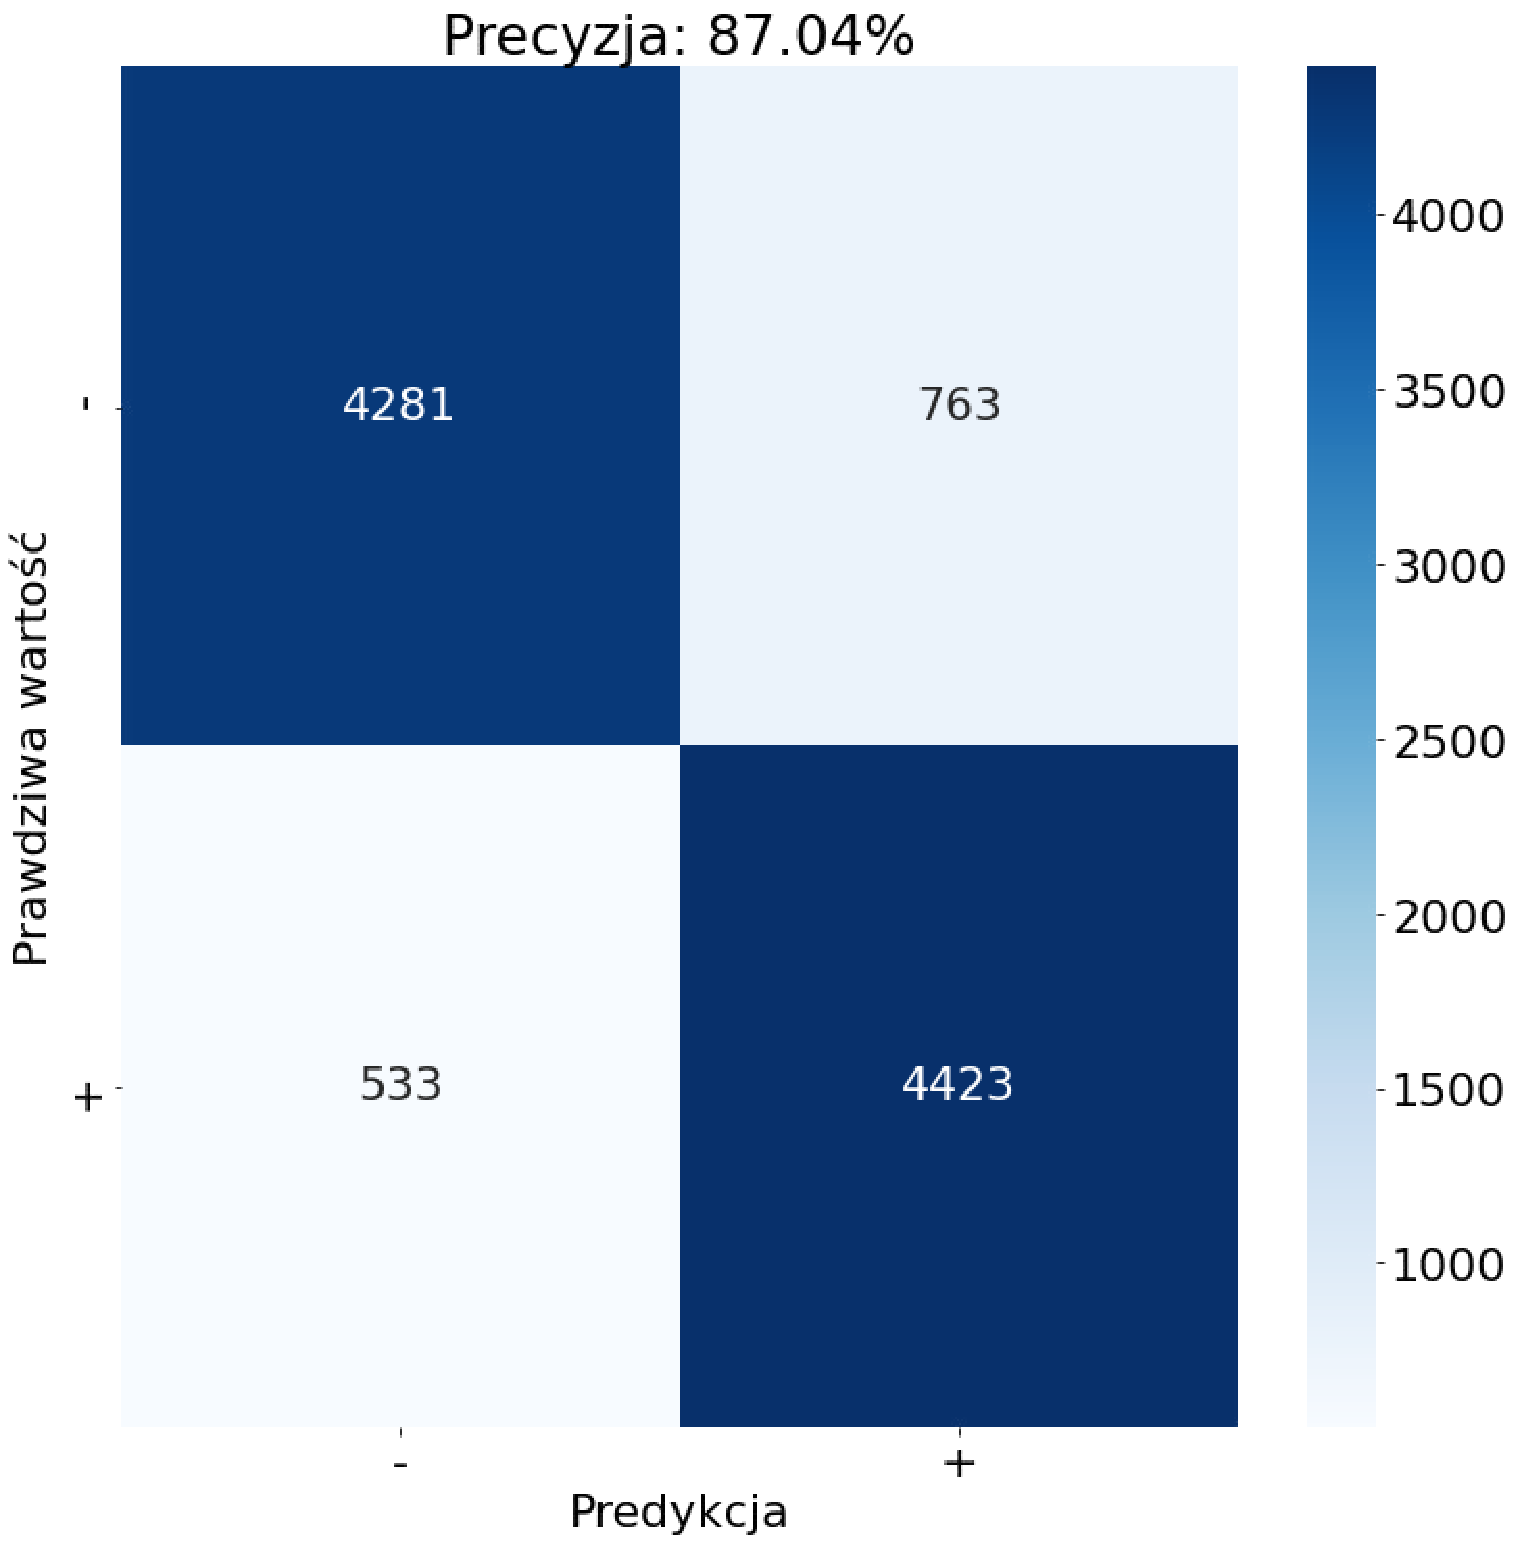
\includegraphics[width=0.5\linewidth]{images/chapter3/rf-macierz.pdf}
	\caption{Wyniki klasyfikacji z użyciem lasu losowego dla n\_estimators=1000 i max\_depth=64. Trening modelu zajął 13.8 minuty.}
	\label{fig:macierz-rf}
\end{figure}

\noindent Kolorem granatowym zostały oznaczone wartości przewidziane prawidłowo przez skonstruowany przez nas model --- 4423 wartości zostały zaklasyfikowane prawidłowo jako pozytywne i 4281 wartości zostały zaklasyfikowane prawidłowo jako negatywne, co po zsumowaniu daje 8704 prawidłowo sklasyfikowane wartości na 10~000 przykładów. Tak więc precyzja predykcji wynosi 87.04\%. Ponadto 763 przykładów zostało błędnie sklasyfikowanych jako pozytywne i 533 błędnie jako negatywne (ćwiartki w kolorze błękitnym). Całkowity czas trenowania modelu zajął tutaj prawie 14 minut. Wydaje się nam, że jest to dosyć długi czas jak na stosunkowo mały (40~000 przykładów) zbiór treningowy.

\noindent W związku z tym, dla porównania wykonałyśmy również analogiczne modelowanie (fitowanie) dla maksymalnej głębokości drzew wynoszącej 32. Czas uległ znacznemu skróceniu. Trenowanie tego samego zbioru zajęło niecałe 4 minuty, a osiągnięta precyzja wyniosła 86.65\%, a więc była tylko o 0.39\% mniejsza niż dla 2$\times$ głębszych drzew. Szczegółowe wyniki przedstawione są w załączonym notatniku Google Colab. Wynik ten wyraźnie sugeruje, że należy się zawsze zastanowić nad sensem dużej głębokości drzew, gdyż w płytszymi drzewami również można osiągnąć zadowalające wyniki, a przy tym znacznie zredukować czas wykonywanych obliczeń.

\noindent Przy pomocy zaimplementowanej przez nas dedykowanej metody (Listing. \ref{code:rf-prior}) został też wyznaczony priorytet cech (\textit{feature importance}), na bazie których następowały podziały w kolejnych węzłach drzew decyzyjnych.

\begin{lstlisting}[language=Python,frame=single, breaklines=true, caption=Metoda do wyznaczania i wizualizacji priorytetu cech dla drzewa decyzyjnego.,label=code:rf-prior]
def plot_feature_importance(model, vectorizer):
	feature_importance = np.array(model.feature_importances_)
	feature_names = np.array(vectorizer.get_feature_names())
	data = pd.DataFrame({'feature_names': feature_names, 'feature_importance': feature_importance})
	
	max_data = data.nlargest(20, ['feature_importance'])
	
	max_data.plot(kind='barh', x='feature_names', y='feature_importance', color=blue_0)
	plt.show()

plot_feature_importance(random_forest_count, count_vectorizer)
\end{lstlisting}


%%%  ------------> obrazek
\begin{figure}[H]
	\centering
	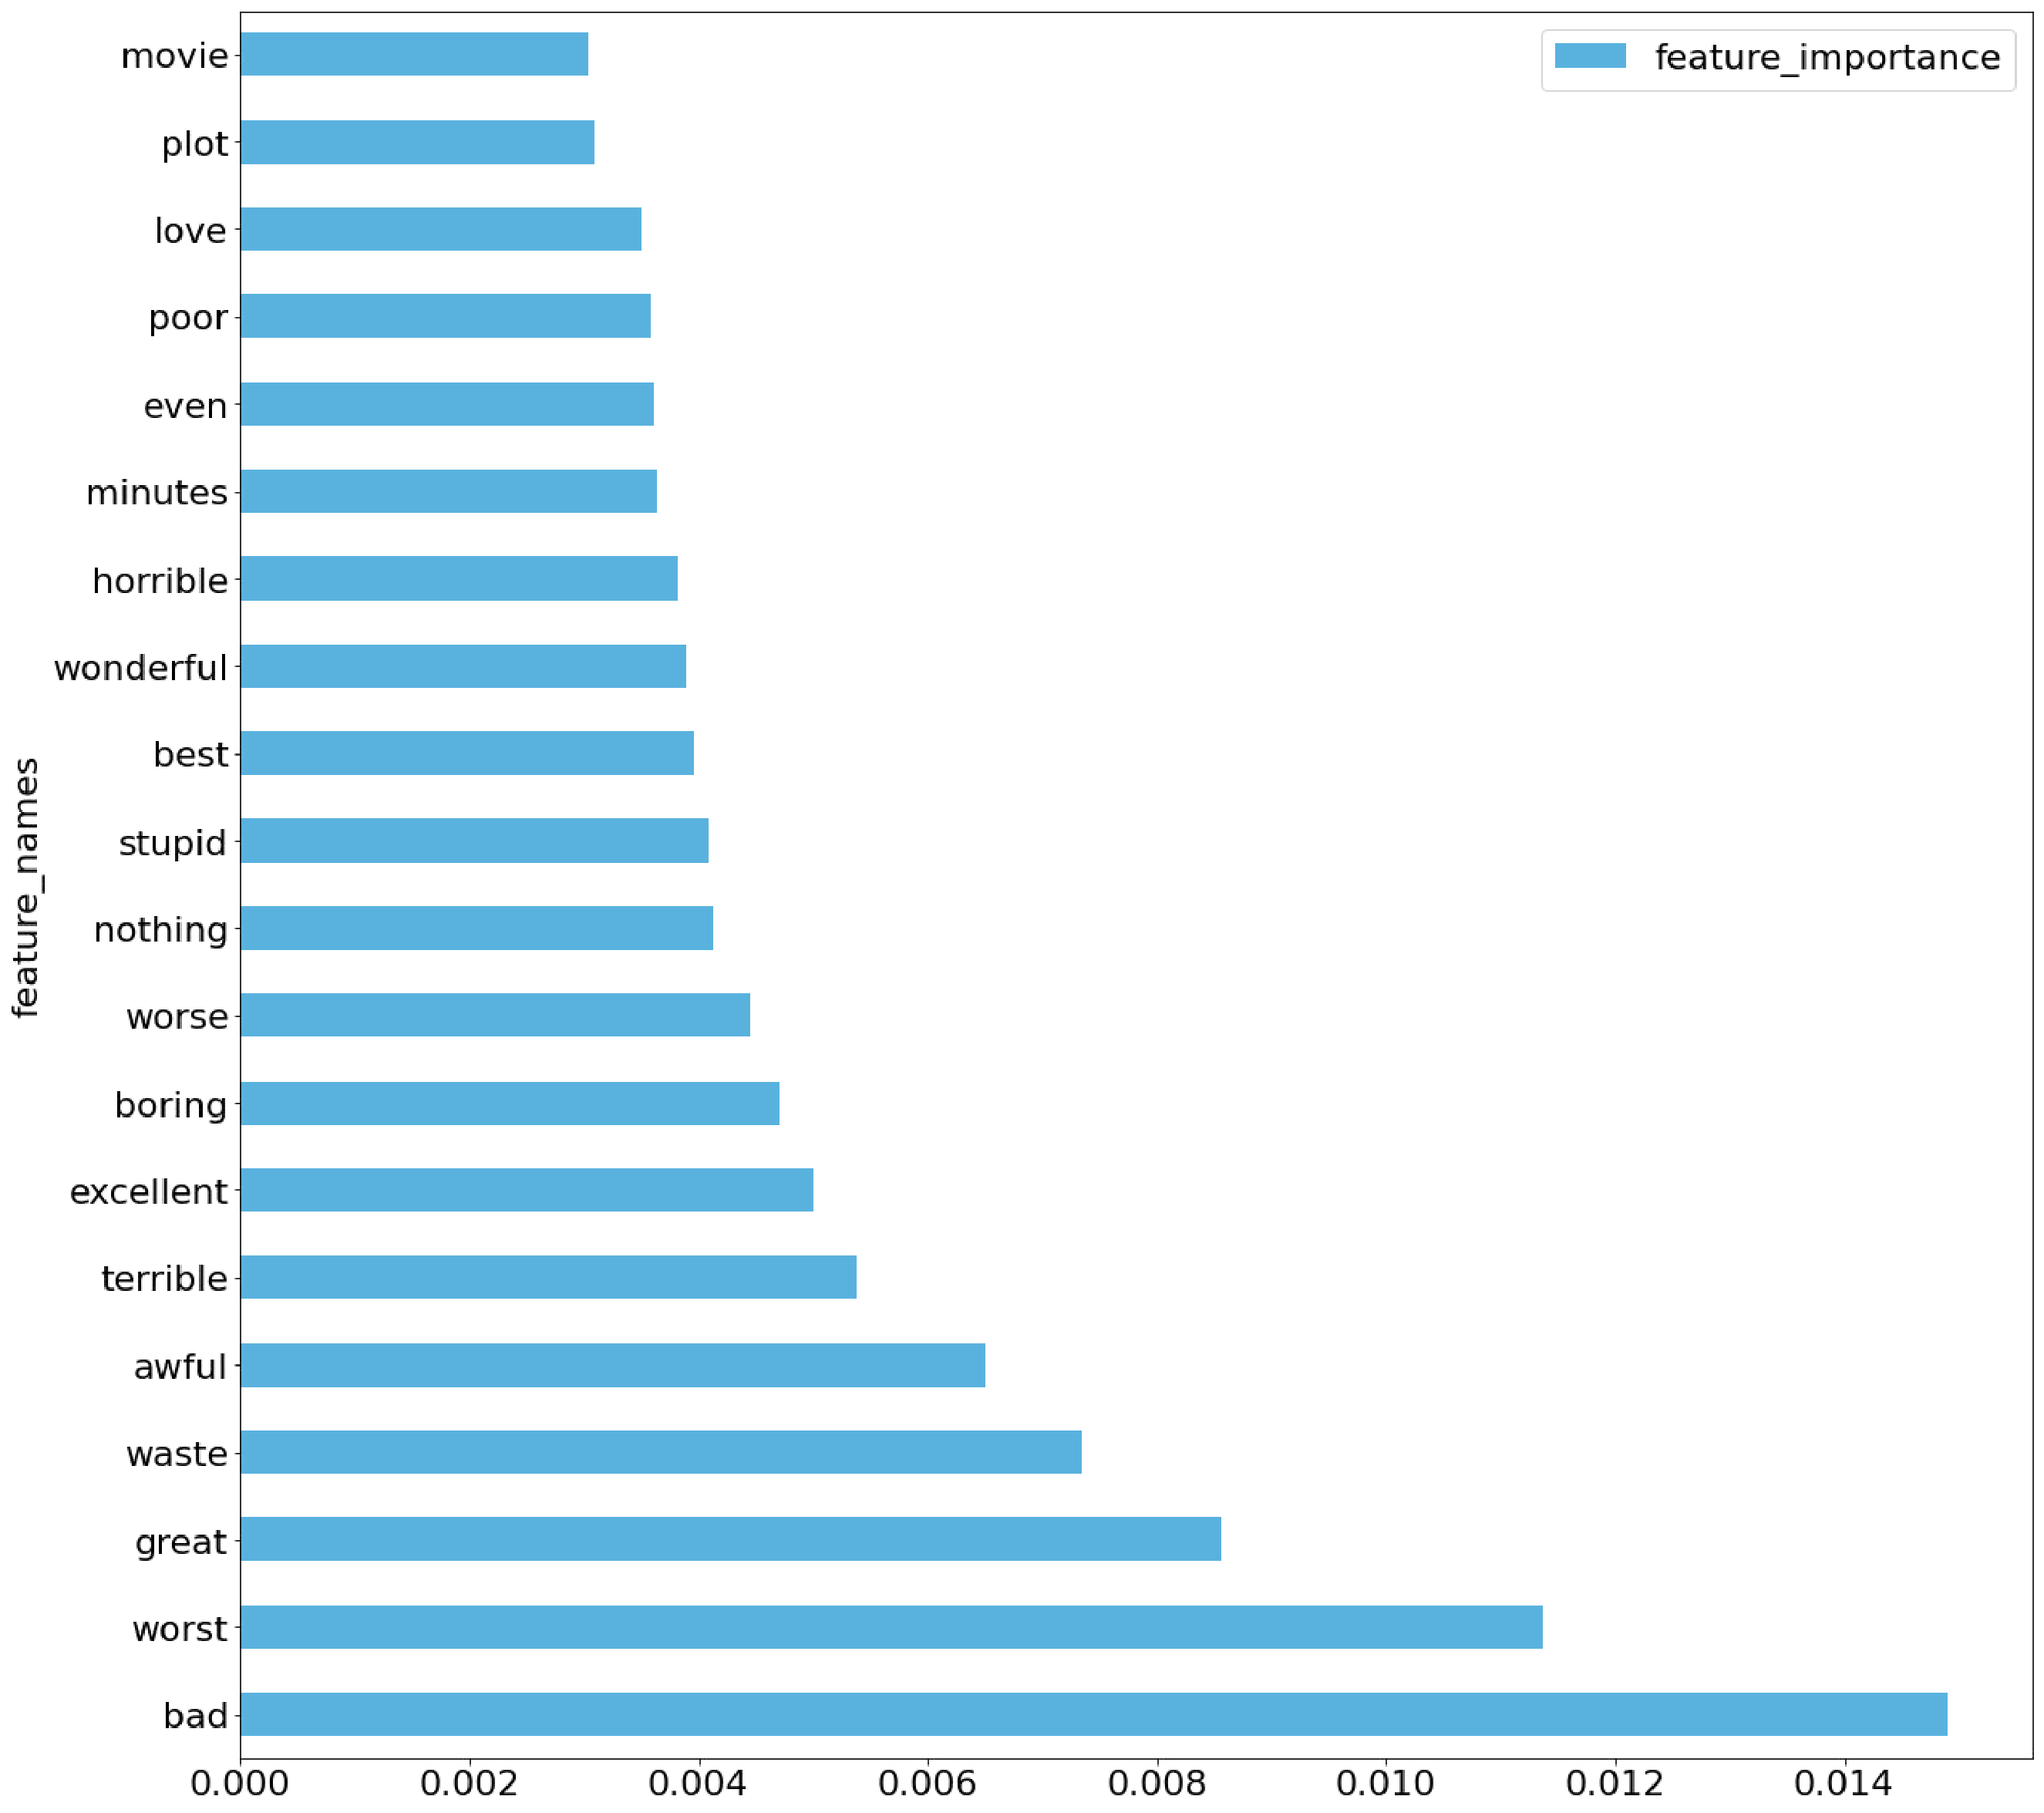
\includegraphics[width=0.55\linewidth]{images/chapter3/rf-feature-import.pdf}
	\caption{Ważność cech w drzewach decyzyjnych.}
	\label{fig:rf-fi}
\end{figure}

\noindent Znalazłysmy też ciekawe narzędzie --- bibliotekę \verb|LIME| --- które umożliwia zwizualizowanie wydźwięków kluczowych słów, które posłużyły do sklasyfikowania danej recenzji jako pozytywnej lub negatywnej. Poszczególne słowa są w tym przypadku oznaczone albo kolorem pomarańczowym (jeżeli są pozytywne) albo niebieskim (gdy są negatywne). Intensywność koloru mówi o tym jak bardzo jwydźwięk ten jest pozytywny lub negatywny. Na poniższym rysunku (Rysunek. \ref{fig:rf-lime}) znajduję się wizualizacja dla przykładowej recenzji pozytywnej (góra) oraz negatywnej (dół).

%%%  ------------> obrazek
\begin{figure}[H]
	\centering
	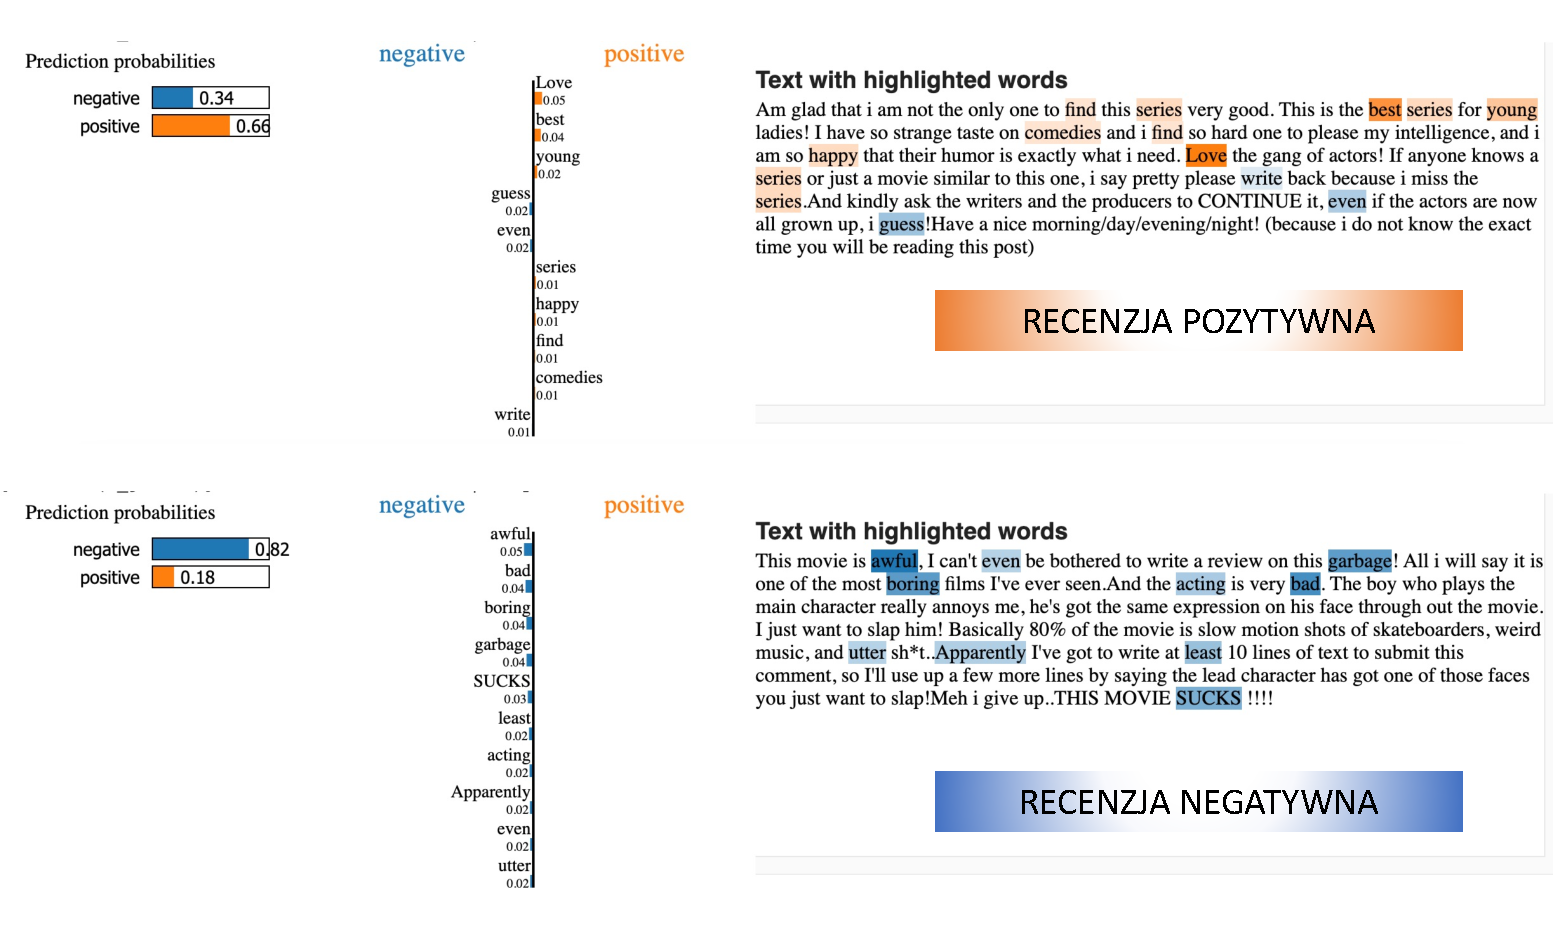
\includegraphics[width=0.8\linewidth]{images/chapter3/rf-lime.pdf}
	\caption{Wykres LIME wydźwięków kluczowych słów dla przykładowej recenzji pozytywnej (góra) oraz negatywnej (dół).}
	\label{fig:rf-lime}
\end{figure}

\noindent Istnieje również możliwość wykonania wizualizacji drzew decyzyjnych, co w prostu sposób pozwala interpretować i wyciągać wnioski. Jednakże głębokość naszych drzew uniemożliwia przedstawienie ich w sposób czytelny, dlatego wizualizacja została pominięta.

\subsection{SVM}
Kolejny model klasyfikacyjny stworzyłyśmy używając klasy \verb|LinearSVC| z pakietu \verb|sklearn.svm|. Dodatkowo przy użyciu klasy \verb|RandomizedSearchCV| oraz  \verb|GridSearchCV| szukałyśmy optymalnego parametru 'C'. Parametr 'C' informuje o tym, jak bardzo chce się uniknąć błędnej klasyfikacji każdego przykładu ze zbioru treningowego \cite{paramC}. Dla dużych wartości 'C' optymalizator wybiera hiperpłaszczyznę o mniejszym marginesie, jeśli ta hiperpłaszczyzna lepiej radzi sobie z prawidłowym sklasyfikowaniem wszystkich punktów treningowych. Przeciwnie, bardzo mała wartość 'C' spowoduje, że optymalizator będzie szukał hiperpłaszczyzny oddzielającej o większym marginesie, nawet jeśli ta hiperpłaszczyzna błędnie zaklasyfikuje większą liczbę punktów (Rysunek. \ref{fig:param-C}). Parametr 'C' jest zasadniczo parametrem regularyzacji, który kontroluje kompromis między osiągnięciem małego błędu dopasowania modelu na danych uczących a minimalizacją norm wag w równaniu modelu.

%%%  ------------> obrazek
\begin{figure}[H]
	\centering
	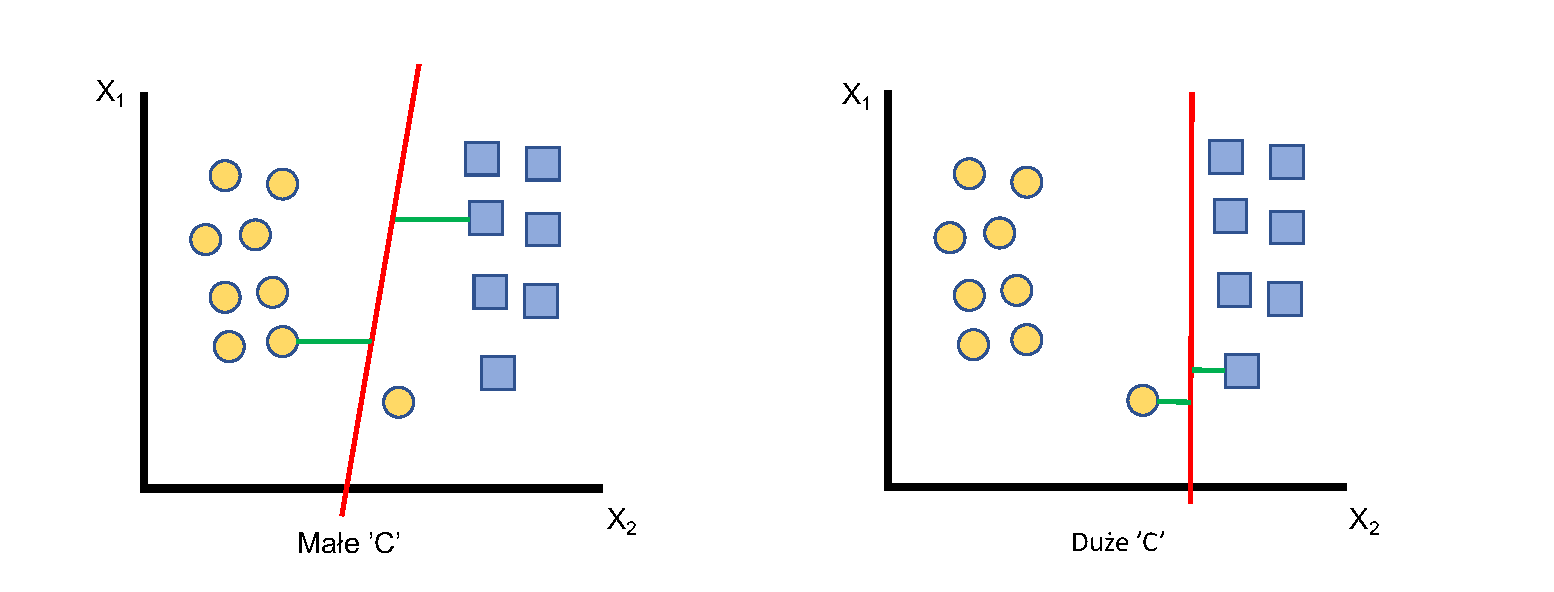
\includegraphics[width=0.85\linewidth]{images/chapter3/param-C.pdf}
	\caption{Idea obrazująca parametr 'C' --- płaszczyzny dla małej (lewy) i dużej (prawy) wartości parametru 'C'.}
	\label{fig:param-C}
\end{figure}


\noindent Pierwsza optymalizacja (SVM\_1) została wykonana z użyciem klasy \verb|RandomizedSearchCV| dla: \verb|params = {'C': scipy.stats.expon(scale=10)}|.


\begin{lstlisting}[language=Python,frame=single, breaklines=true, caption=Modelowanie SVM\_1 (RandomizedSearchCV).,label=code:svm]
from sklearn.svm import LinearSVC
import scipy
from sklearn.model_selection import RandomizedSearchCV

params = {'C': scipy.stats.expon(scale=10)}

grid_count2 = RandomizedSearchCV(LinearSVC(max_iter=5000), params, refit= True, verbose= 3)
grid_count2.fit(train_data_count, train_labels)
param_results = pd.DataFrame(grid_count2.cv_results_)
param_results.sort_values("rank_test_score").head(1)
\end{lstlisting}

\bigskip
\begin{table} [H]
	\caption{Wyniki optymalizacji dla najlepszych iteracji RandomizedSearchCV.}
	\begin{center}
		\begin{tabular}{c  c || c || c  c  c  c  c  || c  || c }
			\hline
			$\overline{t_{fit}}$&$\overline{t_{sc}}$ &\textbf{C} &	sc$_1$&	sc$_2$ &sc$_3$ &	sc$_4$ &	sc$_5$	& \textbf{$\overline{sc}$ }&	$\pm$	\\
			\hline
			10.9&	0.005  & \textbf{0.533} & 0.865 &	0.865 &	0.868 &	0.863 &	0.867 &	\textbf{0.866} &	0.002 \\
			18.2&	0.005&	\textbf{2.29}&	0.861 &	0.862 &	0.864 &	0.856&	0.861&	\textbf{0.861}&	0.002 \\
			\hline
		\end{tabular} \\
		{\scriptsize sc --- score, t --- time (s)}
	\end{center}
\end{table}

\noindent Ze względu na to, że model osiągał znacząco lepsze wyniki z niskimi wartościami parametru 'C', zdecydowałyśmy się na dalszą optymalizację --- tym razem przy użyciu \verb|GridSearchCV| dla: \verb|params = {'C': np.linspace(0, 1, num=1000)}|.

\begin{lstlisting}[language=Python,frame=single, breaklines=true, caption=Modelowanie SVM\_2 (GridSearchCV).,label=code:svm1]
from sklearn.svm import LinearSVC
import scipy
from sklearn.model_selection import GridSearchCV

params = {'C': np.linspace(0, 1, num=1000)}

grid_count2 = GridSearchCV(LinearSVC(max_iter=500),  params, verbose= 3)
grid_count2.fit(train_data_count, train_labels)
param_results = pd.DataFrame(grid_count2.cv_results_)
param_results.sort_values('rank_test_score').head(1)
\end{lstlisting}

\bigskip
\begin{table} [H]
	\caption{Wyniki optymalizacji dla najlepszych iteracji GridSearchCV.}
	\begin{center}
		\begin{tabular}{c  c || c || c  c  c  c  c  || c  || c }
			\hline
			$\overline{t_{fit}}$&$\overline{t_{sc}}$ &\textbf{C} &	sc$_1$&	sc$_2$ &sc$_3$ &	sc$_4$ &	sc$_5$	& \textbf{$\overline{sc}$ }&	$\pm$	\\
			\hline
			0.44&	0.006&	\textbf{0.003}&	0.889 &	0.895 &	0.894 &	0.889&	0.891&	\textbf{0.891}&	0.002 \\
			0.49&	0.006&	\textbf{0.004}&	0.889 &	0.894 &	0.894 &	0.889&	0.891&	\textbf{0.891}&	0.002 \\\\
			\hline
		\end{tabular} \\
		{\scriptsize sc --- score, t --- time (s)}
	\end{center}
\end{table}

\noindent Jak widać, najlepsze wyniki otrzymałyśmy dla parametru 'C', który wynosi $\approx$0.003, a dokładnie 0.00300300300\\3003003, w związku z czym zecydowałyśmy się go użyć w dalszym modelowaniu.
Poniżej znajdują się fragmenty kodu odpowiadające trenowaniu (fitowaniu) modelu \verb|LinearSVC| (Listing. \ref{code:svc-train}) oraz predykcji wartości wyjścia (Listing. \ref{code:svc-pred}).

\bigskip

\begin{lstlisting}[language=Python,frame=single, breaklines=true, caption=Trening SVC dla C 0.003003003003003003.,label=code:svc-train]
svc_classifier_count = LinearSVC(max_iter=500, C=0.003003003003003003)
svc_classifier_count.fit(train_data_count, train_labels)
\end{lstlisting}

\bigskip
\begin{Verbatim}
LinearSVC(
	C=0.003003003003003003,
	class_weight=None,
	dual=True,
	fit_intercept=True, 
	intercept_scaling=1,
	loss='squared_hinge', 
	max_iter=500, 
	multi_class='ovr', 
	penalty='l2', 
	random_state=None, 
	tol=0.0001, 
	verbose=0
	)
\end{Verbatim}

\bigskip
\begin{lstlisting}[language=Python,frame=single, breaklines=true, caption=Predykcja SVC dla C 0.003003003003003003.,label=code:svc-pred]
svc_predictions_count = svc_classifier_count.predict(test_data_count)
print_metrics(svc_predictions_count) # nasza funkcja print_metrics dla CountVectorizera
\end{lstlisting}

\noindent Na rysunku (Rysunek. \ref{fig:macierz-svc}) przedstawiona jest macierz omyłek (pomyłek) zestawiająca wartości prawdziwe oraz te otrzymane w wyniku predykcji wraz z zależnościami pomiędzy nimi.

%%%  ------------> obrazek
\begin{figure}[H]
	\centering
	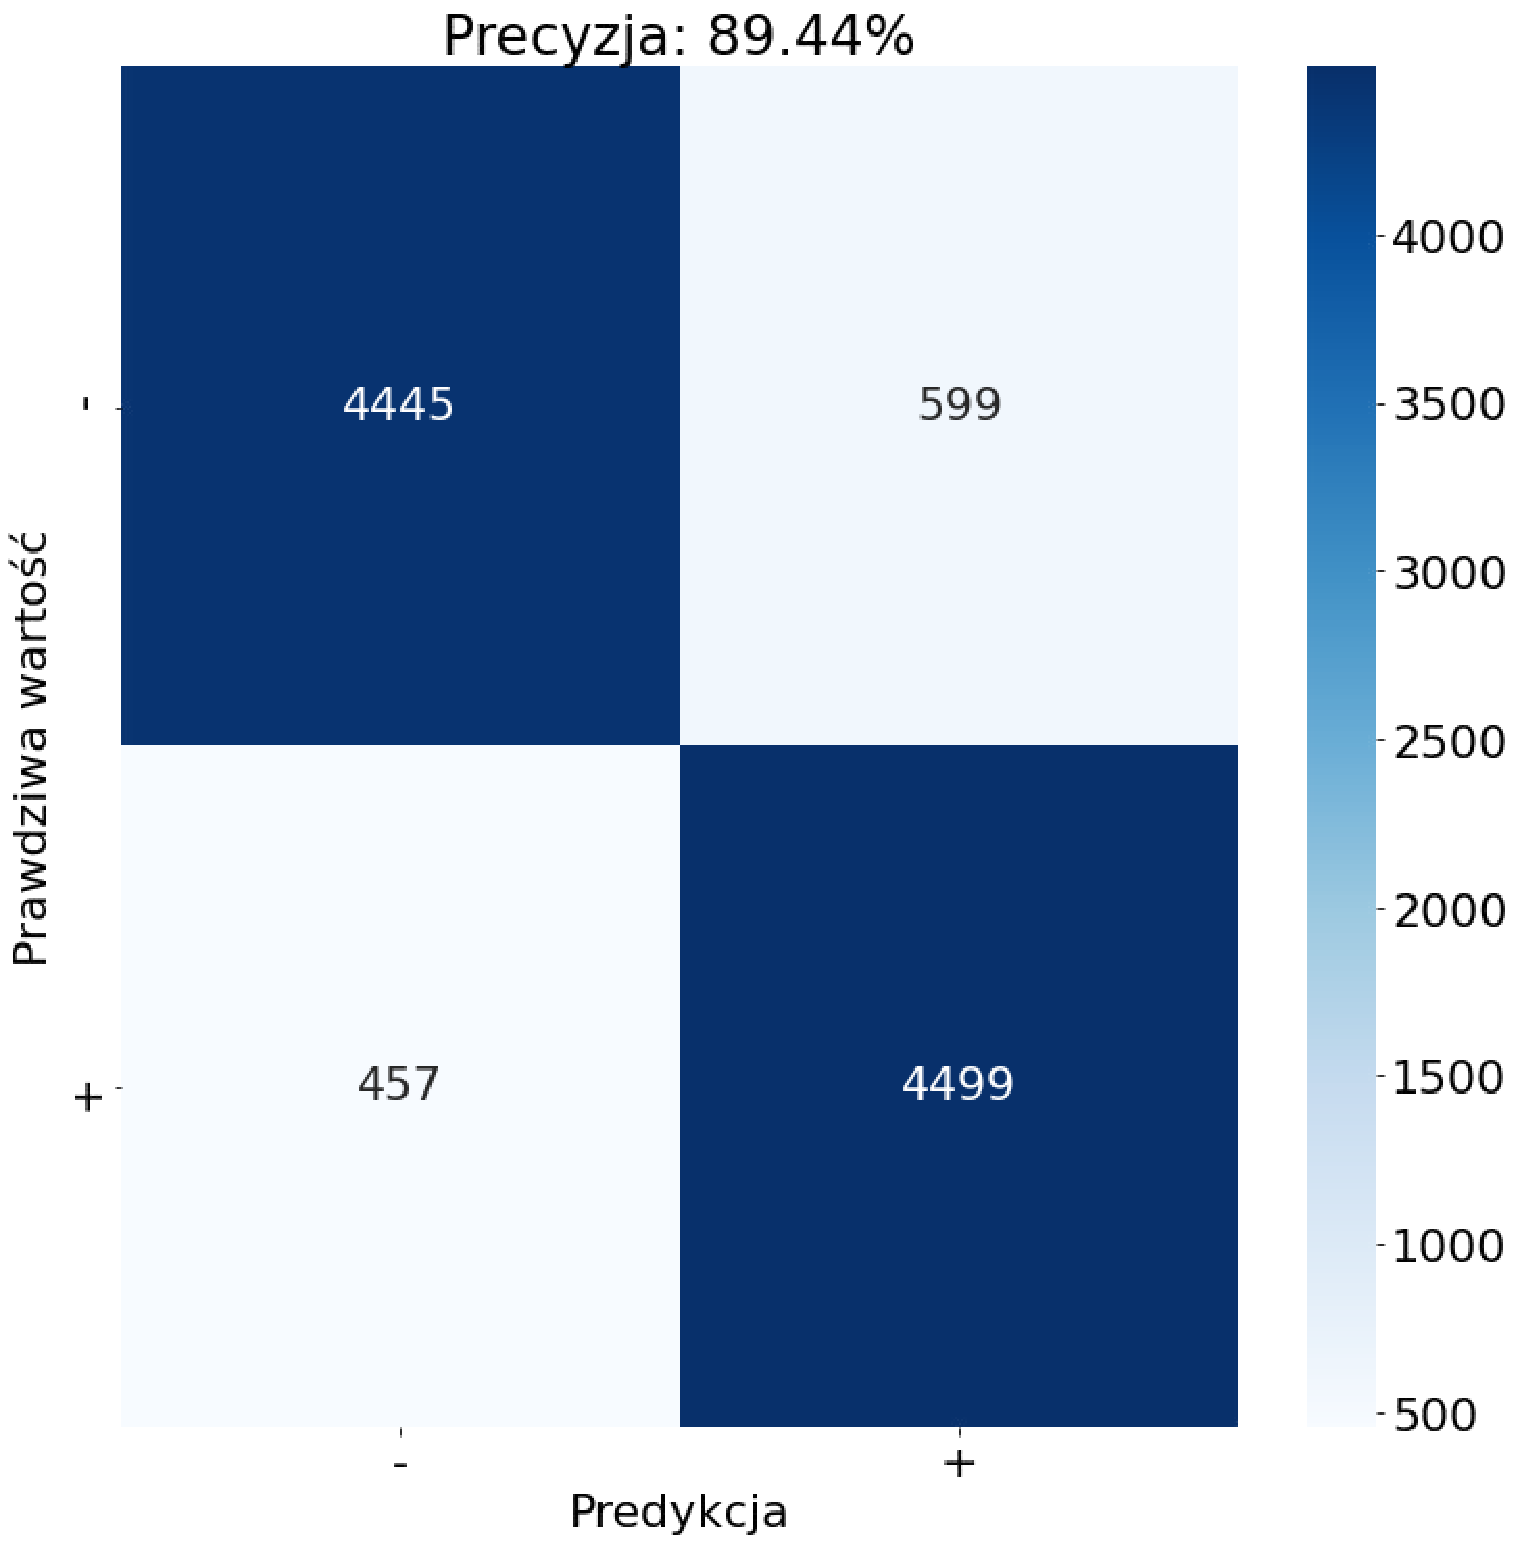
\includegraphics[width=0.5\linewidth]{images/chapter3/svc-macierz.pdf}
	\caption{Wyniki klasyfikacji z użyciem maszyny wektorów nośnych dla parametru C $\approx$ 0.003.}
	\label{fig:macierz-svc}
\end{figure}

\noindent Kolorem granatowym zostały oznaczone wartości przewidziane prawidłowo przez skonstruowany przez nas model --- 4499 wartości zostały zaklasyfikowane prawidłowo jako pozytywne i 4445 wartości zostały zaklasyfikowane prawidłowo jako negatywne, co po zsumowaniu daje 8944 prawidłowo sklasyfikowane wartości na 10~000 przykładów. Tak więc precyzja predykcji wynosi 89.44\%. Wynik wydaje się być logiczny. Ponadto 599 przykładów zostało błędnie sklasyfikowanych jako pozytywne i 457 błędnie jako negatywne (ćwiartki w kolorze błękitnym).

\noindent Na poniższym listingu (Listing. \ref{code:svc-visual}) przedstawiona jest implementacja metody \verb|plot_| \verb|coefficients(...)|, która umożliwia wykonanie wizualizacji najistotniejszych słów po klasyfikacji, które mają wydźwięk negatywny (kolor niebieski) lub pozytywny (kolor różowy).

\begin{lstlisting}[language=Python,frame=single, breaklines=true, caption=Wizualizacja po SVC.,label=code:svc-visual]
from sklearn.feature_extraction.text import CountVectorizer
from sklearn.svm import LinearSVC
import matplotlib.pyplot as plt

def plot_coefficients(classifier, feature_names, top_features=20):
	coef = classifier.coef_.ravel()
	top_positive_coefficients = np.argsort(coef)[-top_features:]
	top_negative_coefficients = np.argsort(coef)[:top_features]
	top_coefficients = np.hstack([top_negative_coefficients, top_positive_coefficients])
	
	# create plot
	plt.figure(figsize=(15, 5))
	colors = [blue_0 if c < 0 else pink_0 for c in coef[top_coefficients]]
	plt.bar(np.arange(2 * top_features), coef[top_coefficients], color=colors)
	feature_names = np.array(feature_names)
	plt.xticks(np.arange(1, 1 + 2 * top_features), feature_names[top_coefficients], rotation=60, ha='right')
	plt.show()

plot_coefficients(svc_classifier_count, count_vectorizer.get_feature_names())	
\end{lstlisting}

%%%  ------------> obrazek
\begin{figure}[H]
	\centering
	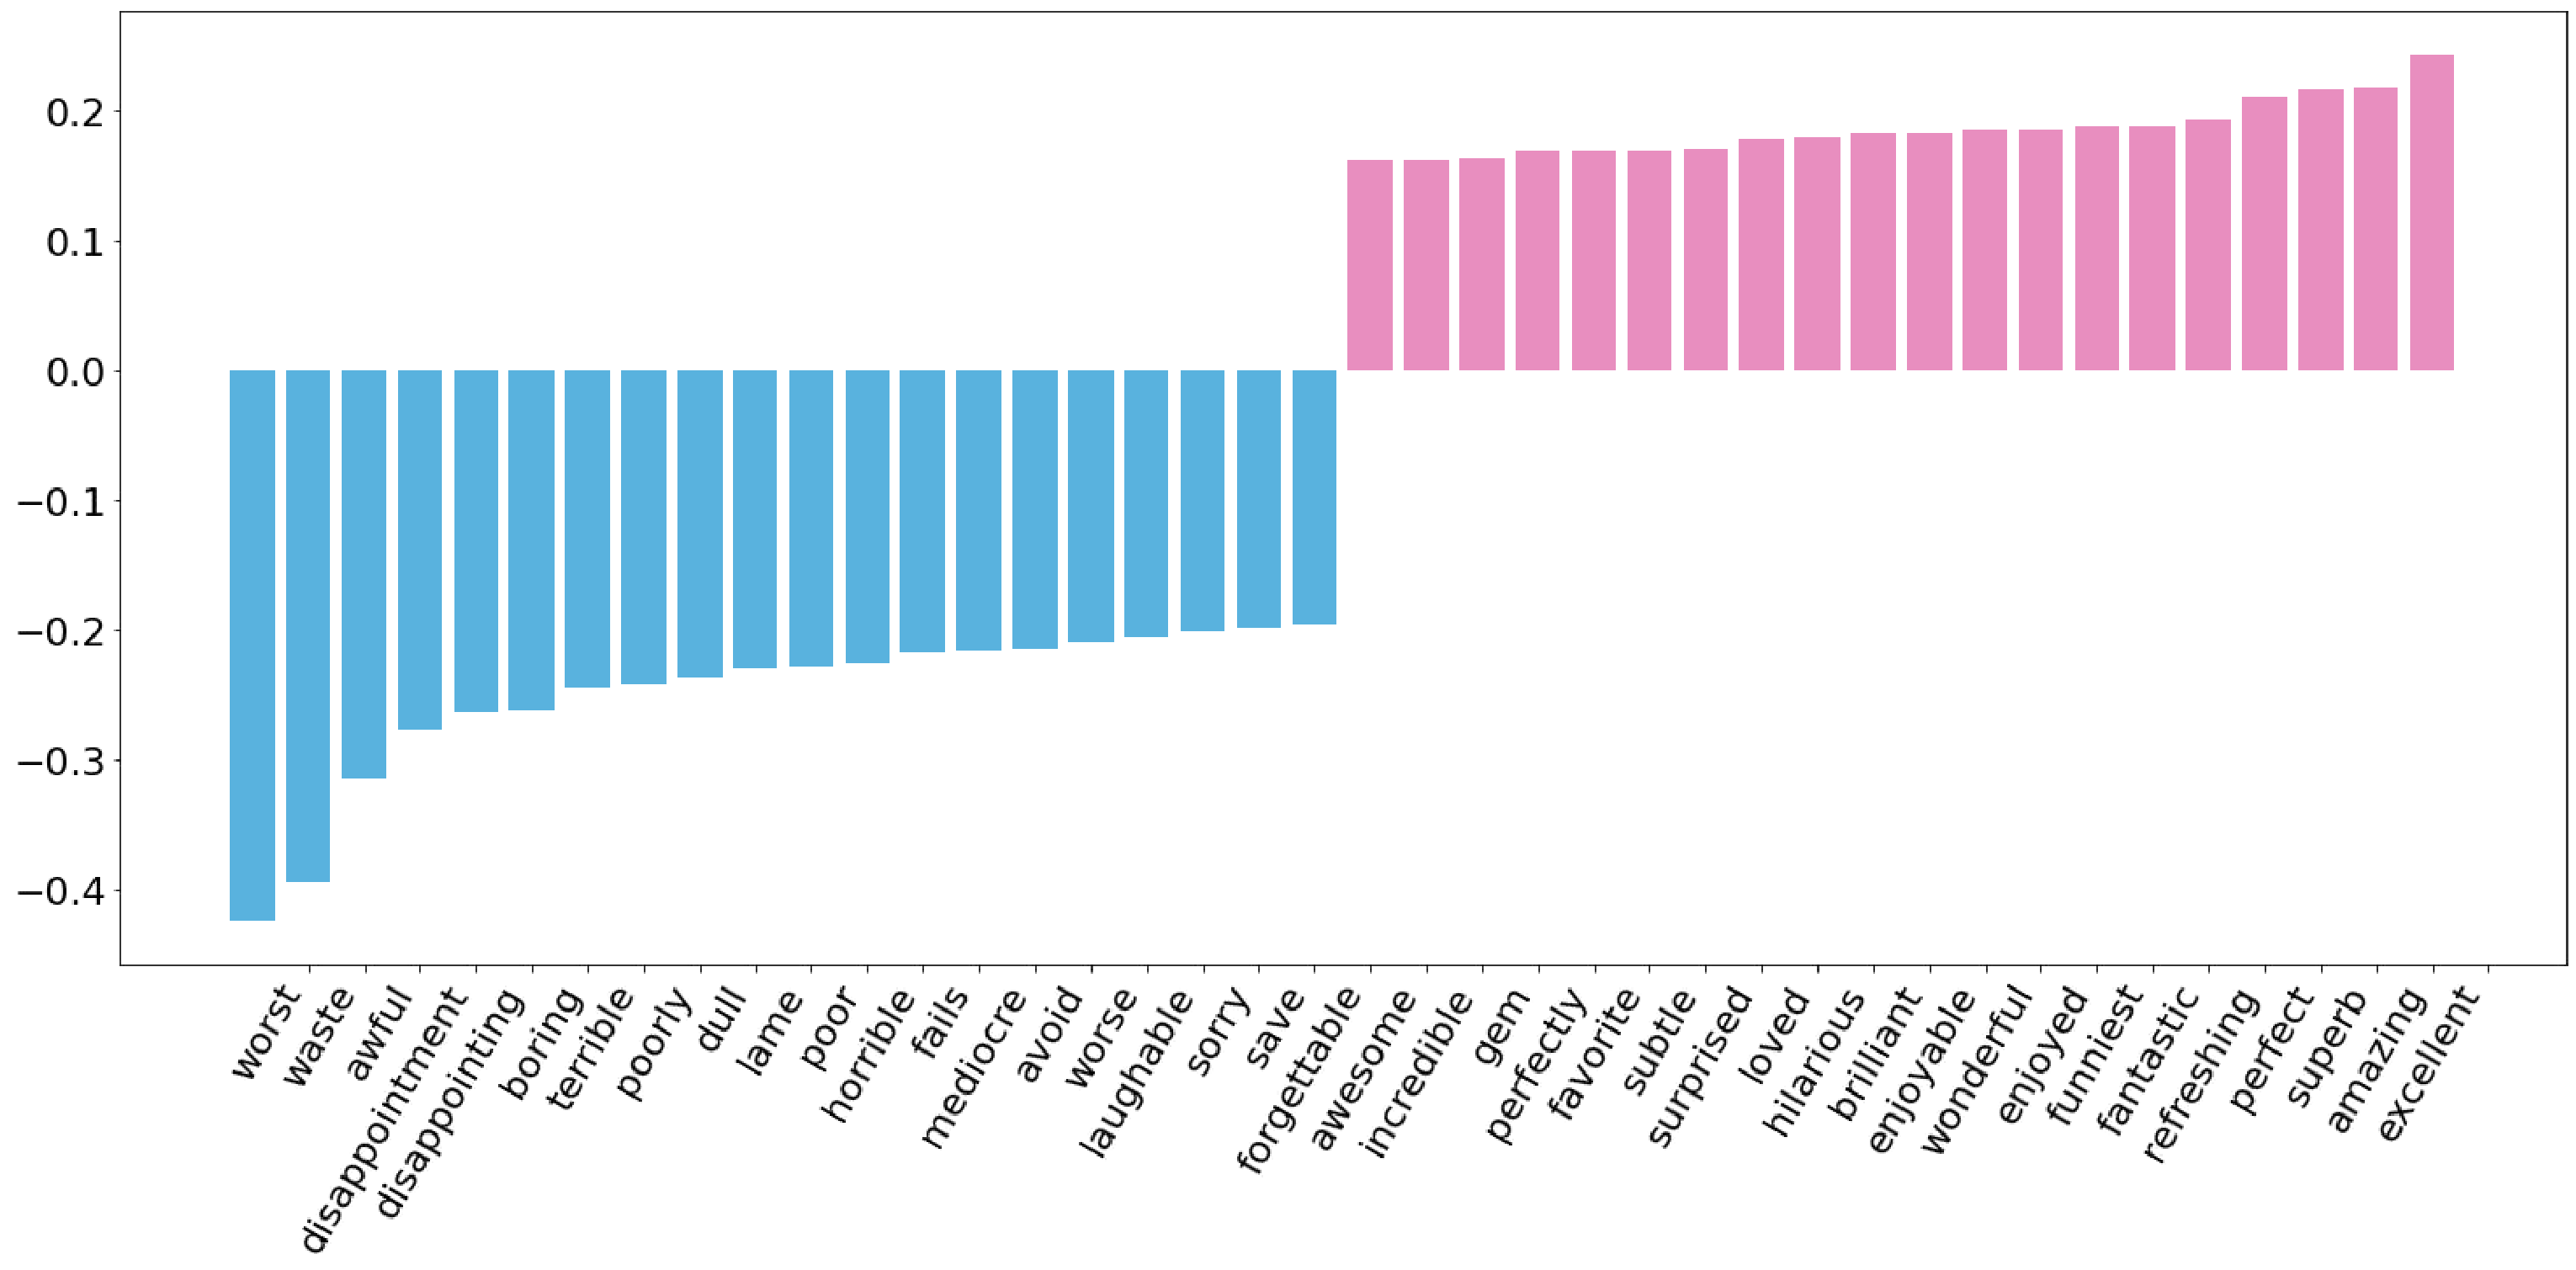
\includegraphics[width=1\linewidth]{images/chapter3/svc-visual.pdf}
	\caption{Wizualizacja wydźwięku pozytywnego lub negatywnego wyrazów (SVC).}
	\label{fig:visual-svc}
\end{figure}



\subsection{Sieci neuronowe}
W kolejnych etapach stworzyłysmy modele sieci neuronowych a dokładniej konwolucyjnej sieci neuronowej (subsekcja \ref{subsec:cnn}), sieci LSTM --- długoterminowej pamięci krótkoterminowej, która jest typem sieci rekurencyjnej (sekcja \ref{sec:lstm}) oraz zamodelowałyśmy wyniki połączenia tych dwóch rodzajów sieci razem (sekcja \ref{sec:cnn-lstm}).

Jako że użycie sieci neuronowych wymaga najpierw wyrażenia każdego słowa w postaci wektora liczb (\textit{embedding}), zastosowałyśmy metodę word2vec \cite{mikolov2013efficient}. Żeby osiągnąć pożądany rezultat zaimplementowałysmy metodą \verb|get_lists_of_words(data)|, do której zaaplikowałyśmy nasze dane treningowe i w rezultacie otrzymałyśmy listę słów.

\begin{lstlisting}[language=Python,frame=single, breaklines=true, caption=Stworzenie listy słów dla modelu Word2Vec.,label=code:w2v-wordlist]
import re
def get_lists_of_words(data):
	clean_reviews = data.map(lambda review: re.sub(r'([^a-z|\s])+', '', review.lower()))
	return [review.split() for review in clean_reviews]

train_data_list_of_words = get_lists_of_words(train_data)
\end{lstlisting}	

\noindent Następnie wytrenowałysmy model \verb|Word2Vec| na tej stworzonej liście słów.
\begin{lstlisting}[language=Python,frame=single, breaklines=true, caption=Trenowanie modelu Word2vec.,label=code:w2v]
import gensim
word2vec_model = gensim.models.Word2Vec(
				train_data_list_of_words,
				size=150,  
				window=10, 
				min_count=2, 
				workers=10
				)

word2vec_model.train(train_data_list_of_words,total_examples=len(train_data_list_of_words),epochs=10)
\end{lstlisting}

\noindent Wytrenowane wektory słów są przechowywane w instancji KeyedVectors jako, w naszym przypadku, \verb|word2vec_model.wv|. Ten obiekt zasadniczo zawiera mapowanie między słowami i osadzaniami/ zagłębieniami (\textit{embeddings}).


\noindent Pakiet gensim zapewnia też wiele przydatnych metod. Na przykład dzięki metodzie \verb|most_similar('słowo')| umożliwia znajdowanie słów najbardziej zbliżonych do podanego w parametrze słowa (Listing. \ref{code:similar-different}, linia 1) oraz dzięki metodzie \verb|doesnt_match| \verb|([słowa])| słowo/a, które nie pasuje/ą do reszty słów na liście (Listing. \ref{code:similar-different}, linia 2).

\begin{lstlisting}[language=Python,frame=single, breaklines=true, caption=Znajdowanie najbardziej zbliżonych i niepasujących słów.,label=code:similar-different]
Linia 1:   word2vec_model.wv.most_similar('actor')
Linia 2:   word2vec_model.wv.doesnt_match(['good', 'nice','small', 'fine'])
\end{lstlisting}

\noindent Słowa najbardziej zbliżone do słowa actor:
\begin{Verbatim}
[('actress', 0.5977960824966431),
('performer', 0.5925692915916443),
('role', 0.5761367678642273),
('comedian', 0.5694815516471863),
('performance', 0.5201245546340942),
('newcomer', 0.4978533387184143),
('actors', 0.4970739483833313),
('impersonation', 0.47669658064842224),
('thespian', 0.47024333477020264),
('foxx', 0.46994471549987793)]
\end{Verbatim}

\noindent Słowo nie pasujące do reszty:
\begin{Verbatim}
small
\end{Verbatim}

\begin{lstlisting}[language=Python,frame=single, breaklines=true, caption=Generacja wektora słów --- model Word2Vec.,label=code:w2v-results]
word_vectors = pd.DataFrame(word2vec_model[word2vec_model.wv.vocab], word2vec_model.wv.vocab)
\end{lstlisting}

%%%  ------------> obrazek
\begin{figure}[H]
	\centering
	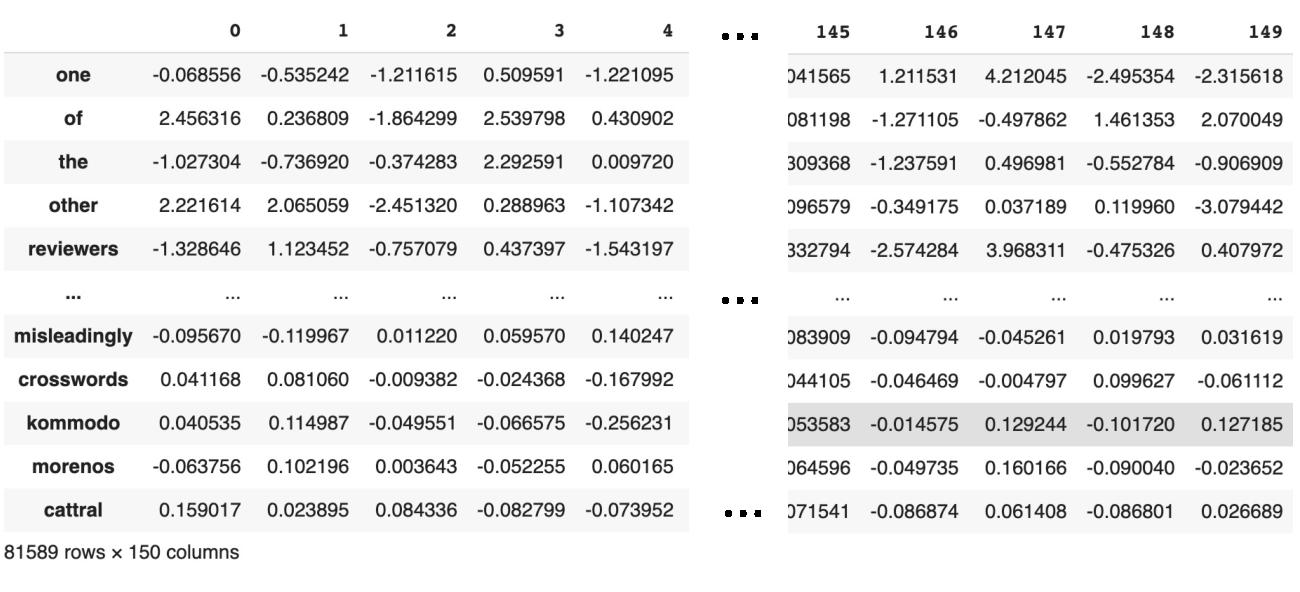
\includegraphics[width=1\linewidth]{images/chapter3/w2v-dframe.pdf}
	\caption{Wyniki modelu Word2Vec --- wektory słów, dla size=150.}
	\label{fig:w2v-dframe}
\end{figure}

\noindent Rezultaty działania modelu można również wizualizować, ale najpierw należy zmniejszyć wymiarowość wektorów --- w naszym przypadku ze 150 wymiarów do 2. Można to zrobić przy użyciu klasy \verb|TSNE| z pakietu \verb|sklearn.manifold| (Listing. \ref{code:tsne}), która pozwoli wygenerować odpowiednie punkty, które można później przedstawić w formie wykresu.

\begin{lstlisting}[language=Python,frame=single, breaklines=true, caption=Zmniejszenie wymiarowości wektorów słów do punktów.,label=code:tsne]
from sklearn.manifold import TSNE
tsne = TSNE(perplexity = 30, n_components=2, init='pca', n_iter=50000, method='exact')tsne = TSNE(perplexity = 30, n_components=2, init='pca', n_iter=50000, method='exact')

points = tsne.fit_transform(np.array(word_vectors)[1000:1500,:])
\end{lstlisting}

\noindent Możliwe jest wygenerowanie wykresu/ grafiki, na której zaznaczone są słowa (wszystkie lub wybrany podzbiór). Słowa o podobnym znaczeniu powinny tworzyć skupiska --- znajdować się blisko siebie. Jednakże, jeżeli stworzy się taką grafikę dla zbyt dużej liczby słów, to staje się ona mało czytelna. Idea tej wizualizacji dla 500 przykładowych słów z naszego zbioru znajduje się poniżej (Rysunek. \ref{fig:w2v-kropki}). Jak widać, przy tym powiększeniu grafika ta jest mało użyteczna. Po odpowiednim (dużym) powiększeniu można znaleźć pewne skupiska słów i zależności.

%%%  ------------> obrazek
\begin{figure}[H]
	\centering
	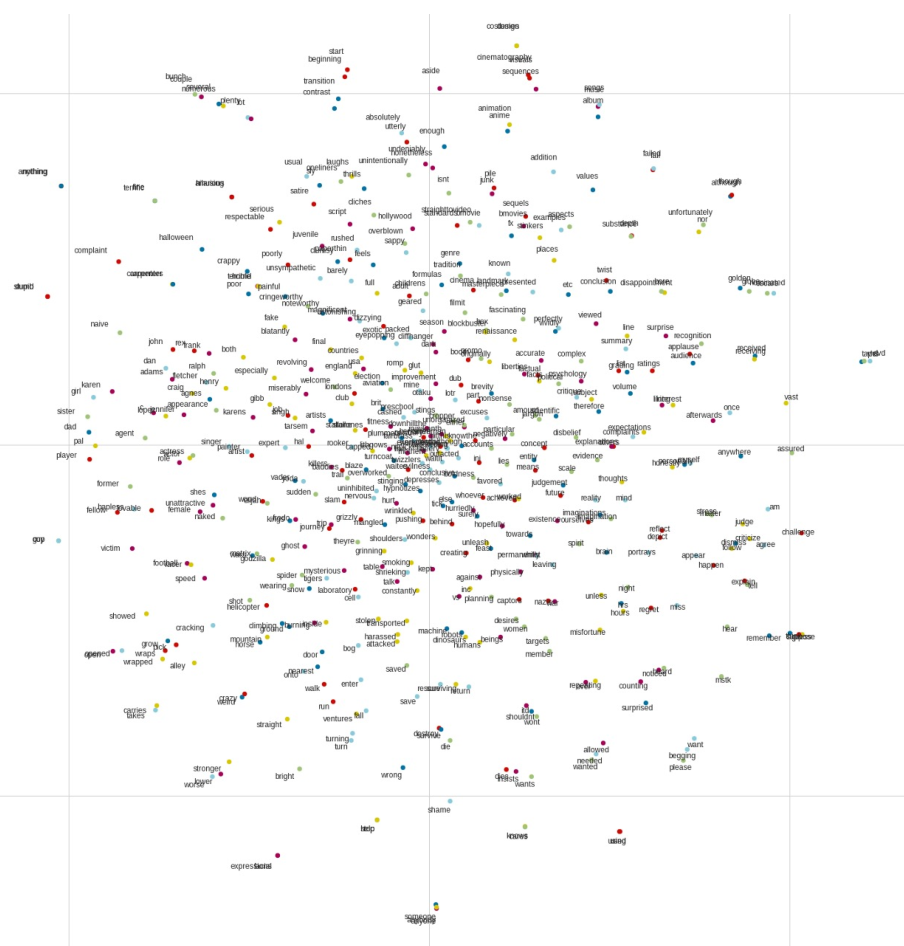
\includegraphics[width=0.95\linewidth]{images/chapter3/w2v-kropki.pdf}
	\caption{Wizualizacja W2V}
	\label{fig:w2v-kropki}
\end{figure}


\noindent Podobnie może być przydatny również rozkład długości recenzji (wyrażony jako liczba słów w recenzji).  Taką zależnośc również można zwizualizować z zaznaczeniem wybranych percentyli (Rysunek. \ref{fig:w2v-percentyle}). W naszym przypadku łatwo zauważyć, że połowa recenzji ma 170 słów lub mniej, 25\% recenzji ma długość między 171 a 273 słowa, kolejne 15\% recenzji ma długość pomiędzy 274 a 441 słów, a 10\% jest dłuższych niż 441 słów. Wyraźnie dominują tu recenzje krótkie. W sumie 75\% recenzji jest co najwyżej średniej długości (do 273 słów).

%%%  ------------> obrazek
\begin{figure}[H]
	\centering
	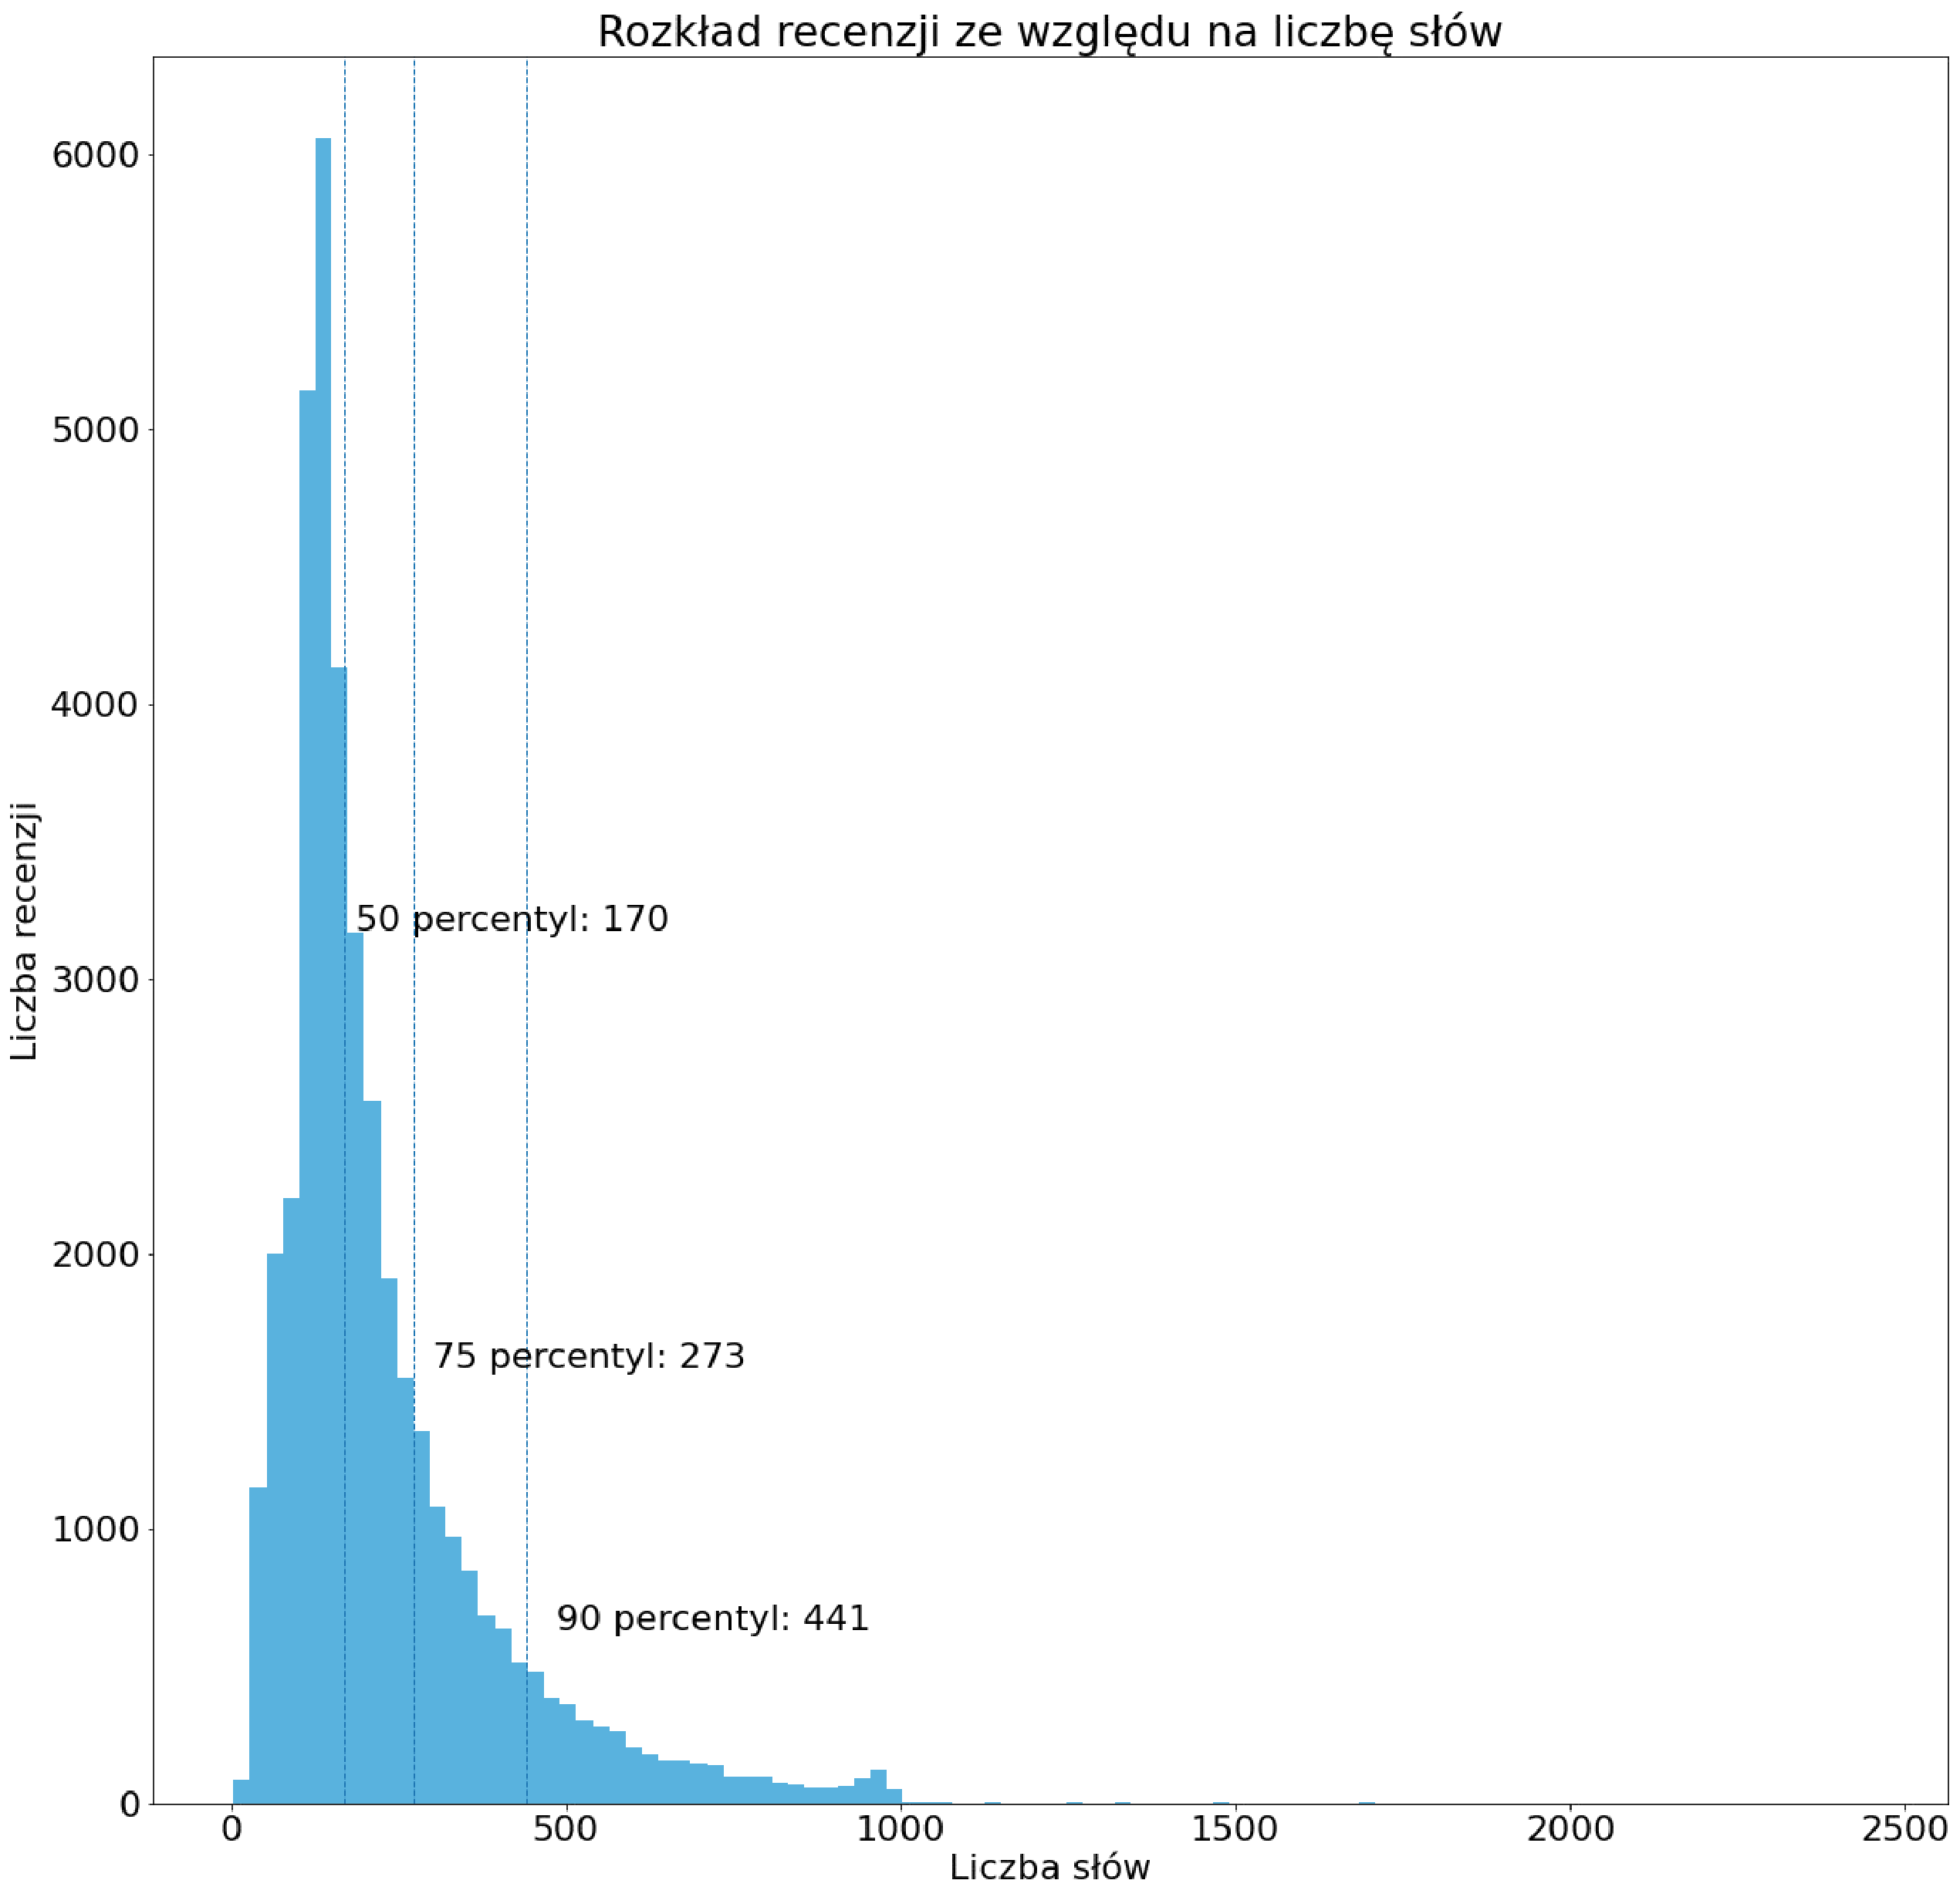
\includegraphics[width=0.75\linewidth]{images/chapter3/w2v-percentyle.pdf}
	\caption{Wizualizacja rozkładu liczby słów w recenzjach.}
	\label{fig:w2v-percentyle}
\end{figure}

\noindent Tak więc tworząc macierze danych do trenowania modeli sieci neuronowych ustaliłyśmy 273 słowa jako górną granicę (maksymalny wymiar).

\subsection{Konwolucyjna sieć neuronowa}

\noindent W wyniku wykonania szeregu przekształceń (dokładna procedura znajduje się w notebooku Google Colab w części Data Preparation dla sieci neuronowych) otrzymałyśmy dwie macierze danych treningową --- \verb|train_data_matrix| i testową --- \verb|test_data_matrix|.
Następnie zdefiniowałysmy funkcję \verb|cnn_model| i przy użyciu biblioteki \verb|keras| stworzyłyśmy model konwolucyjnej sieci neuronowej. W warstwie konwolucyjnej wykorzystałyśmy 128 filtrów o długości 5 oraz funkcję aktywacji ReLu. Następnie, wykorzystałyśmy warstwę \textit{global max pooling} oraz \textit{dropout} z prawdopodobieństwen 0.2.  Użyłyśmy również 10 warstw ukrytych z funkcją aktywacji ReLu oraz ostatniej warstwy wyjściowej z sigmoidalną warstwą aktywacji (dokładne parametry na Listingu. \ref{code:cnn}). Jako funkcji straty użyłyśmy \verb|binary_crossentropy|,a metryką sukcesu ponownie zostało \verb|accuracy|.

\begin{lstlisting}[language=Python,frame=single, breaklines=true, caption=Model CNN.,label=code:cnn]
def cnn_model():
	embed_size=150
	model = Sequential()
	model.add(layers.Embedding(embedding_matrix_size + 1, embed_size, weights=[embedding_matrix]))
	model.add(layers.Conv1D(128, 5, activation='relu'))
	model.add(layers.GlobalMaxPooling1D())
	model.add(layers.Dropout(0.2))
	model.add(layers.Dense(10, activation='relu'))
	model.add(layers.Dense(1, activation='sigmoid'))
	
	model.compile(loss='binary_crossentropy',
	metrics=['accuracy'])
	
	return model
\end{lstlisting}

\begin{Verbatim}
Model: 'Sequential'
Layer (type)                 Output Shape              Param #   
=================================================================
embedding_6 (Embedding)      (None, None, 150)         10894350  
_________________________________________________________________
conv1d_6 (Conv1D)            (None, None, 128)         96128     
_________________________________________________________________
global_max_pooling1d_6 (Glob (None, 128)               0         
_________________________________________________________________
dropout_4 (Dropout)          (None, 128)               0         
_________________________________________________________________
dense_12 (Dense)             (None, 10)                1290      
_________________________________________________________________
dense_13 (Dense)             (None, 1)                 11        
=================================================================
Total params: 10,991,779
Trainable params: 10,991,779
Non-trainable params: 0
\end{Verbatim}

\noindent Powyższy model został skompilowany. Jak widać składa się z prawie 11 milionów trenowalnych parametrów, a następnie wytrenowany. 

\begin{lstlisting}[language=Python,frame=single, breaklines=true, caption=Trening modelu CNN.,label=code:cnn-trening]
cnn_model = cnn_model().fit(
			train_data_matrix,
			train_labels,
			epochs=8,
			verbose=True,
			batch_size=100
			)
\end{lstlisting}

\begin{Verbatim}
Epoch 1/8 - 169s 418ms/step - loss: 0.5815 - accuracy: 0.6748
Epoch 2/8 - 166s 416ms/step - loss: 0.3491 - accuracy: 0.8466
Epoch 3/8 - 166s 415ms/step - loss: 0.2954 - accuracy: 0.8750
Epoch 4/8 - 166s 414ms/step - loss: 0.2593 - accuracy: 0.8930
Epoch 5/8 - 166s 415ms/step - loss: 0.2279 - accuracy: 0.9069
Epoch 6/8 - 165s 412ms/step - loss: 0.1989 - accuracy: 0.9192
Epoch 7/8 - 164s 409ms/step - loss: 0.1729 - accuracy: 0.9316
Epoch 8/8 - 165s 412ms/step - loss: 0.1499 - accuracy: 0.9415
\end{Verbatim}

\noindent Ostatnią czynnością jaką zrobiłyśmy dla tego modelu była predykcja klas w oparciu o zbiór testowy (Listing. \ref{code:cnn-pred}).

\begin{lstlisting}[language=Python,frame=single, breaklines=true, caption=Predykcja z użyciem modelu CNN.,label=code:cnn-pred]
cnn_predictions = cnn_model.predict_classes(test_data_matrix)
\end{lstlisting}

\noindent Wyniki przedstawione są w macierzy omyłek (Rysunek. \ref{fig:cnn-macierz}).

\noindent Kolorem granatowym zostały oznaczone wartości przewidziane prawidłowo przez skonstruowany przez nas model --- 4412 wartości zostały zaklasyfikowane prawidłowo jako pozytywne i 4512 wartości zostały zaklasyfikowane prawidłowo jako negatywne, co po zsumowaniu daje 8924 prawidłowo sklasyfikowane wartości na 10~000 przykładów. Tak więc precyzja predykcji wynosi 89.24\%. Ponadto 532 przykładów zostało błędnie sklasyfikowanych jako pozytywne i 544 błędnie jako negatywne (ćwiartki w kolorze błękitnym). Całkowity czas trenowania modelu zajął tutaj nieco ponad 22 minuty (średnio około 2 minuty i 46 sekund na 1 epokę). Jest to czas dłuższy niż dla dotychczasowych dwóch modeli, ale trzeba tu podkreślić, że model ten posiadał prawie 11 milionów trenowalnych parametrów.
%%%  ------------> obrazek
\begin{figure}[H]
	\centering
	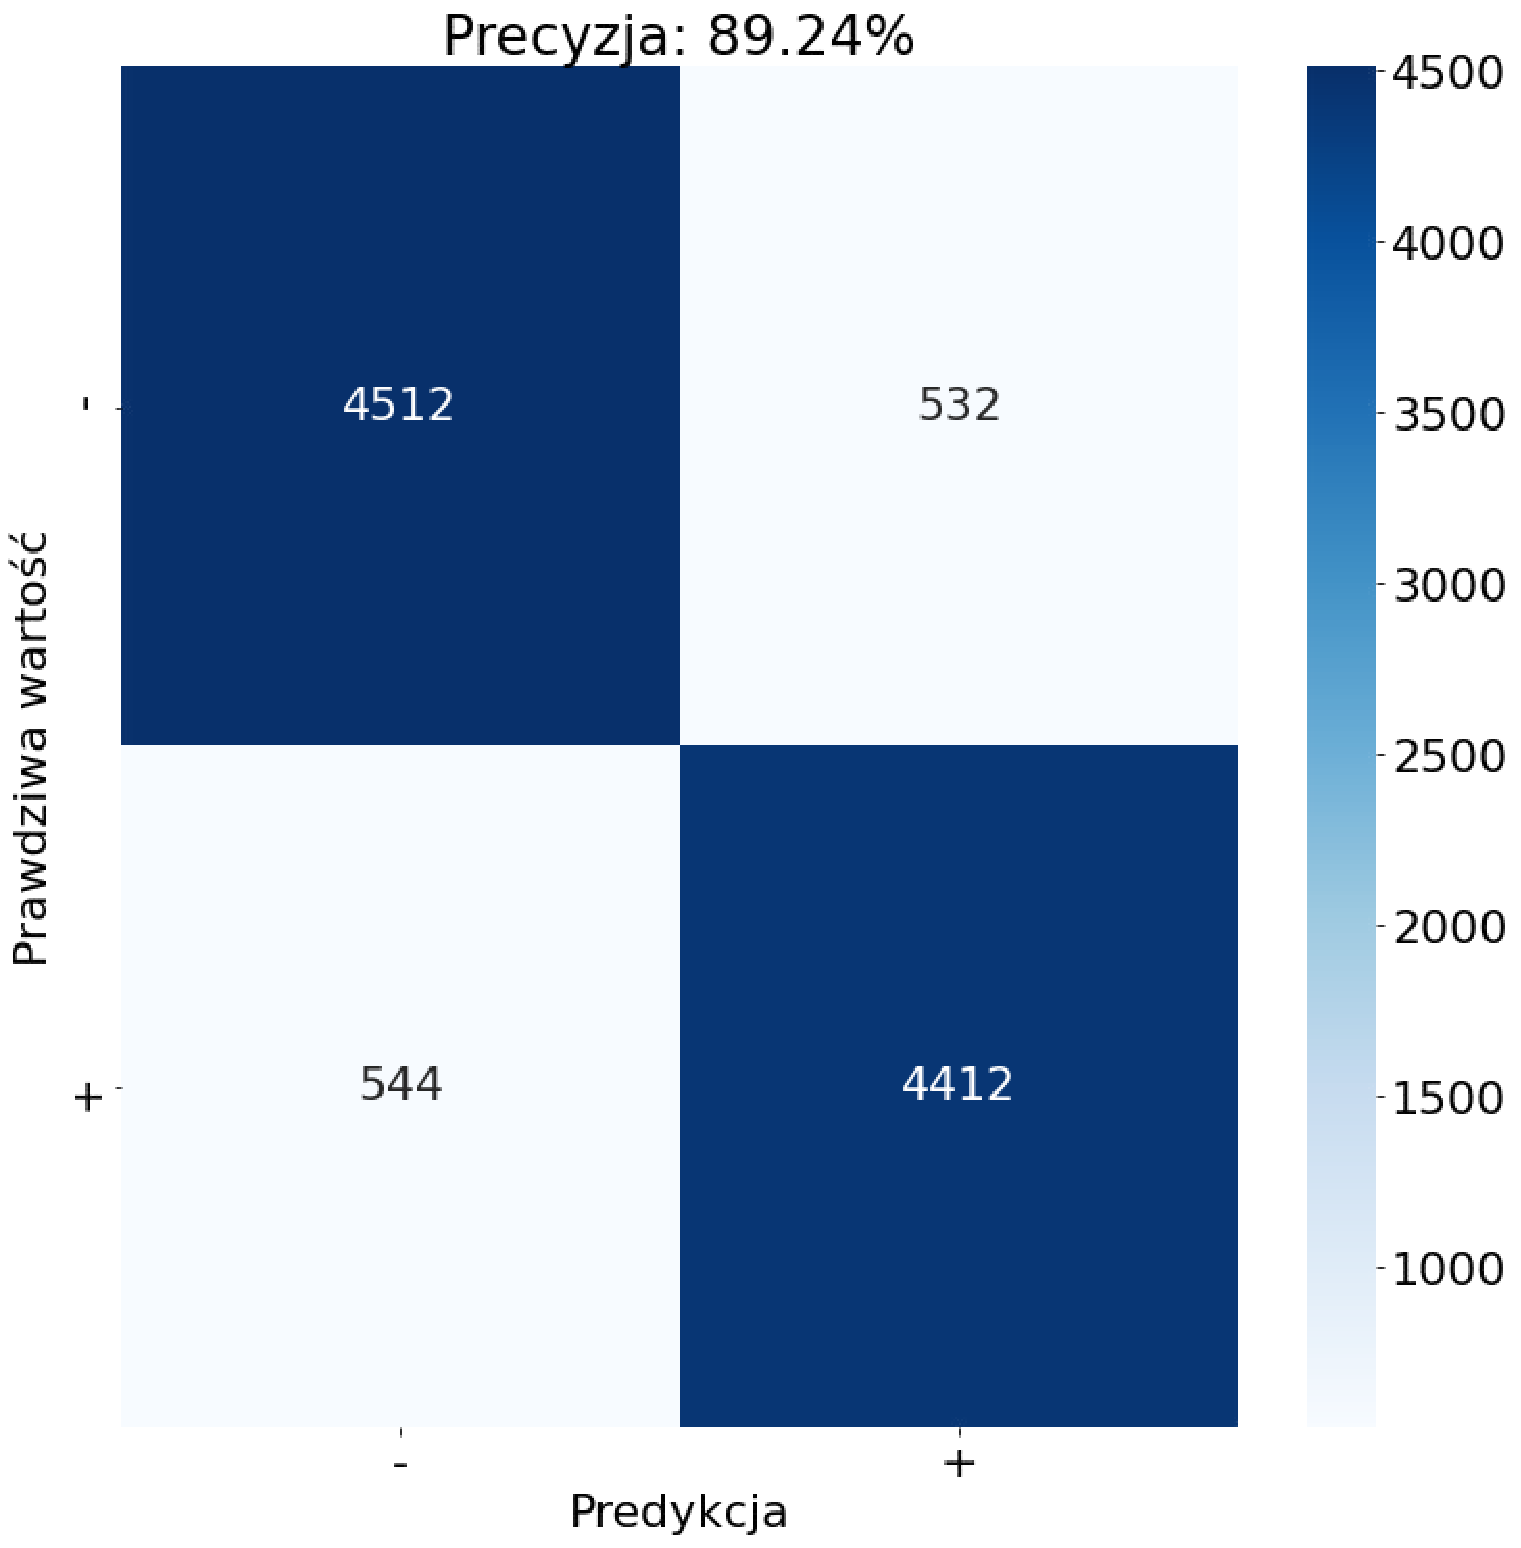
\includegraphics[width=0.5\linewidth]{images/chapter3/cnn-macierz.pdf}
	\caption{Wyniki klasyfikacji z użyciem konwolucyjnej sieci neuronowej.}
	\label{fig:cnn-macierz}
\end{figure}




%----------------- LSTM ----------------
\subsection{LSTM}

Model LSTM został zaimplementowany podobnie jak model konwolucyjny z użyciem \verb|Sequential()|. Zdefiniowałyśmy funkcję \verb|model_lstsm| i przy użyciu biblioteki \verb|keras| stworzyłyśmy model sieci neuronowej LSTM. Zamiast warstwy konwolucyjnej, używamy tutaj warstwy LSTM z wektorem wyjściowym o długości 128. Jako że jest to model rekurencyjny ustawiłyśmy dodatkowy parametr \verb|recurrent_dropout| na wartość 0.2. Ostatnia warstwa --- wyjściowa ma sigmoidalną aktywację (dokładne parametry na Listingu. \ref{code:lstm}). Jako funkcji straty ponownie użyłyśmy \verb|binary_crossentropy|, a jako metryki sukcesu \verb|accuracy|.

\begin{lstlisting}[language=Python,frame=single, breaklines=true, caption=Model LSTM.,label=code:lstm]
def lstsm_model():
	embed_size=150
	model = Sequential()
	model.add(layers.Embedding(embedding_matrix_size + 1, embed_size, weights=[embedding_matrix]))
	model.add(layers.LSTM(128, dropout=0.2, recurrent_dropout=0.2))
	model.add(layers.Dense(1, activation='sigmoid'))
	print(model.summary())
	model.compile(loss='binary_crossentropy',
	metrics=['accuracy'])
	return model
\end{lstlisting}

\newpage
\begin{Verbatim}
Model: 'Sequential'
Layer (type)                 Output Shape              Param #   
=================================================================
embedding_4 (Embedding)      (None, None, 150)         10894350  
_________________________________________________________________
lstm (LSTM)                  (None, 128)               142848    
_________________________________________________________________
dense_8 (Dense)              (None, 1)                 129       
=================================================================
Total params: 11,037,327
Trainable params: 11,037,327
Non-trainable params: 0
\end{Verbatim}


\noindent Powyższy model został skompilowany. Jak widać składa się z ponad 11 milionów trenowalnych parametrów, a następnie wytrenowany. 

\begin{lstlisting}[language=Python,frame=single, breaklines=true, caption=Trening modelu LSTM.,label=code:lstm-trening]
lstm_model = lstsm_model().fit(
			train_data_matrix,
			train_labels,
			epochs=8,
			verbose=True,
			batch_size=100
			)
\end{lstlisting}

\begin{Verbatim}
Epoch 1/8 - 583s 1s/step - loss: 0.5784 - accuracy: 0.6985
Epoch 2/8 - 576s 1s/step - loss: 0.4081 - accuracy: 0.8310
Epoch 3/8 - 583s 1s/step - loss: 0.3197 - accuracy: 0.8699
Epoch 4/8 - 577s 1s/step - loss: 0.2765 - accuracy: 0.8904
Epoch 5/8 - 575s 1s/step - loss: 0.2416 - accuracy: 0.9055
Epoch 6/8 - 577s 1s/step - loss: 0.2169 - accuracy: 0.9155
Epoch 7/8 - 569s 1s/step - loss: 0.1934 - accuracy: 0.9259
Epoch 8/8 - 564s 1s/step - loss: 0.1702 - accuracy: 0.9358
\end{Verbatim}

\noindent Ostatnią czynnością jaką zrobiłyśmy dla tego modelu była predykcja klas w oparciu o zbiór testowy (Listing. \ref{code:cnn-pred}).

\begin{lstlisting}[language=Python,frame=single, breaklines=true, caption=Predykcja z użyciem modelu LSTM.,label=code:lstm-pred]
lstm_predict_data = lstm_model.predict(test_data_matrix)
\end{lstlisting}

Poniżej przedstawiłyśmy macierz omyłek.

\begin{figure}[H]
	\centering
	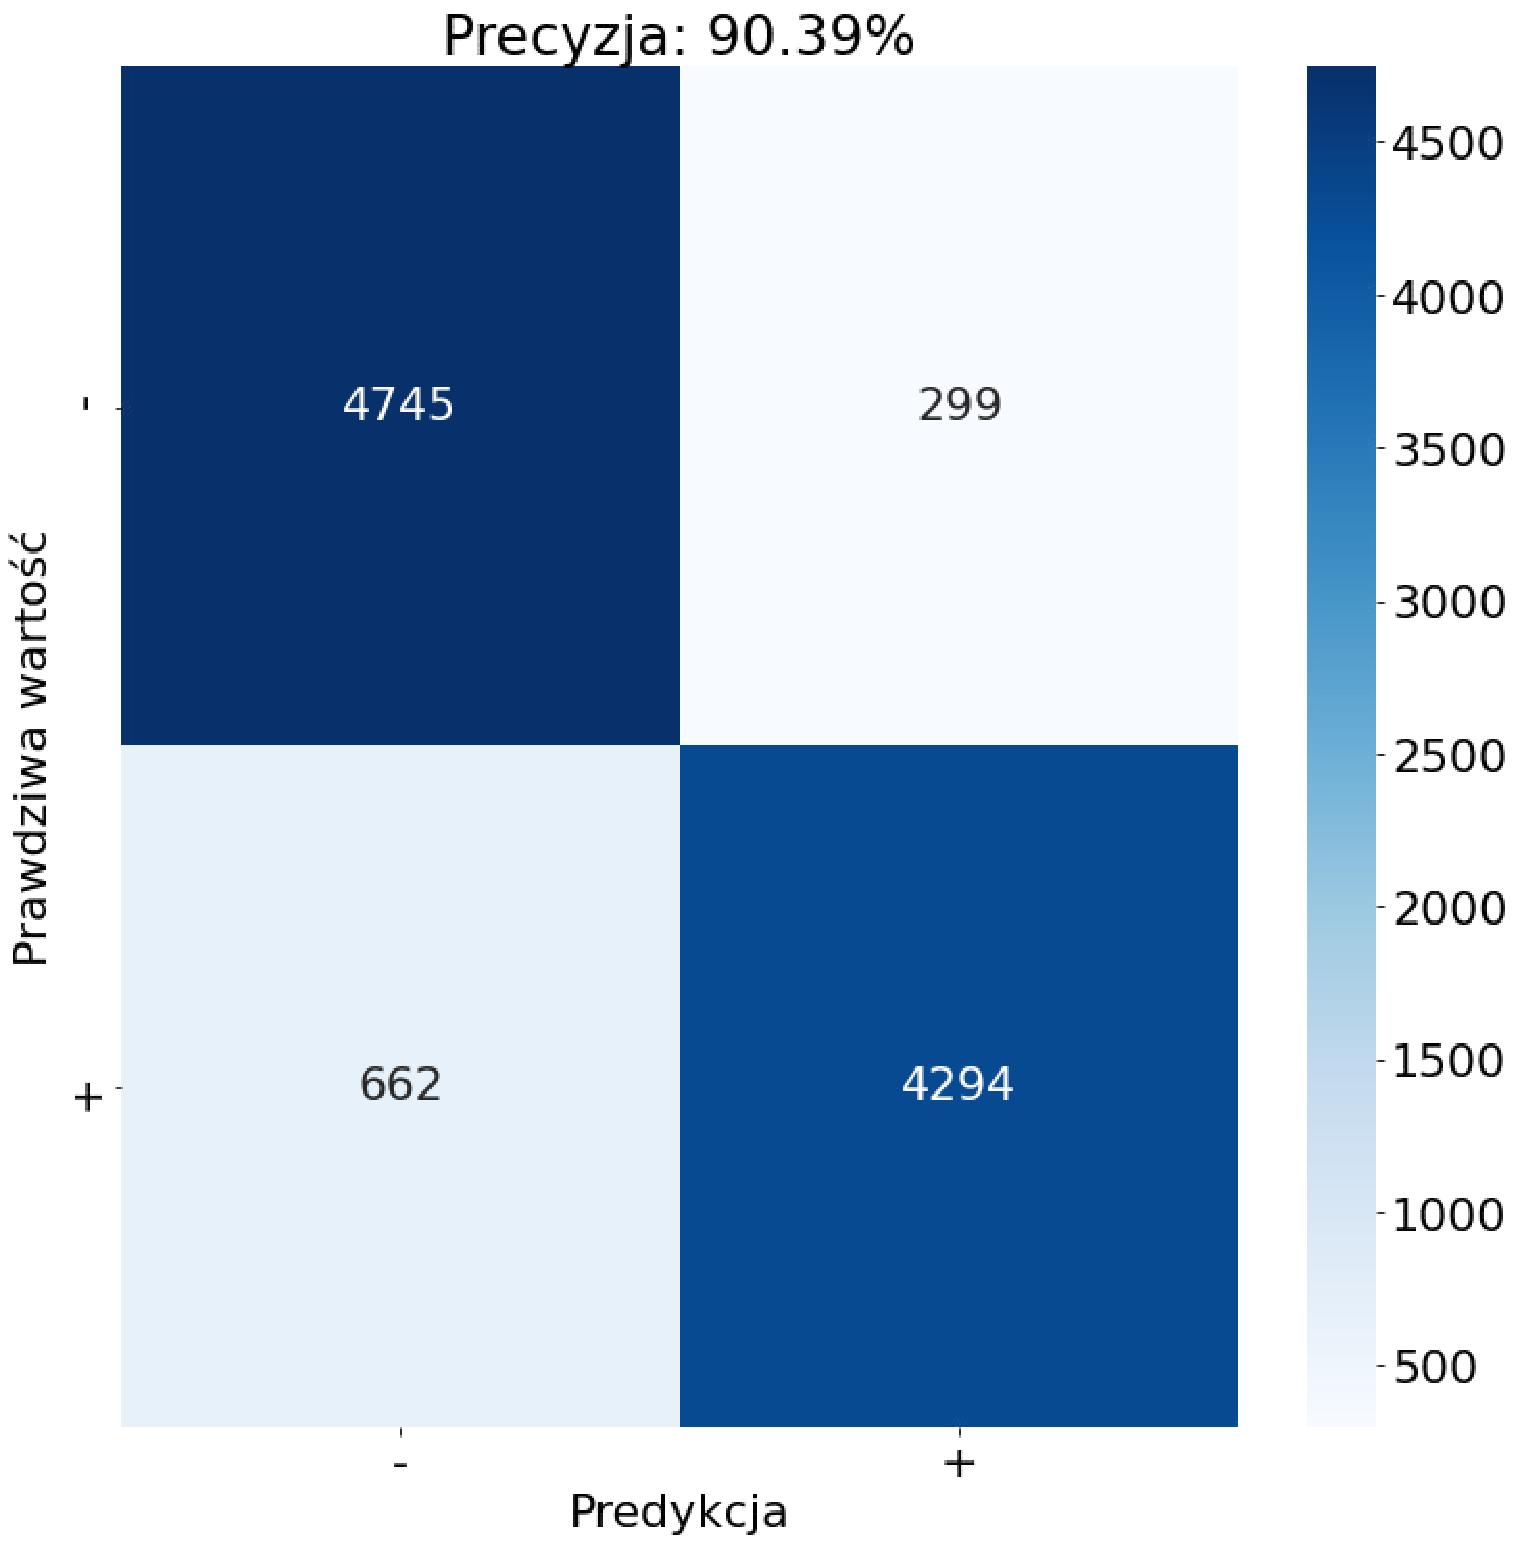
\includegraphics[width=0.5\linewidth]{images/chapter3/lstm-macierz.pdf}
	\caption{Wyniki klasyfikacji z użyciem sieci LSTM.}
	\label{fig:lstm-macierz}
\end{figure}

\noindent Kolorem granatowym zostały oznaczone wartości przewidziane prawidłowo przez skonstruowany przez nas model --- 4294 wartości zostały zaklasyfikowane prawidłowo jako pozytywne i 4745 wartości zostały zaklasyfikowane prawidłowo jako negatywne, co po zsumowaniu daje 9039 prawidłowo sklasyfikowane wartości na 10~000 przykładów. Tak więc precyzja predykcji wynosi 90.39\%. Ponadto 299 przykładów zostało błędnie sklasyfikowanych jako pozytywne i 662 błędnie jako negatywne (ćwiartki w kolorze błękitnym). Całkowity czas trenowania modelu zajął tutaj ponad 76 minut (średnio około 9 minut i 35 sekund na 1 epokę). Jest to czas znacznie dłuższy niż dla dotychczasowych modeli --- lecz model jest również najbardziej zaawansowany i składa się z ponad 11 mln parametrów.


%--------------- CNN-LSTM Ensemble -------------
\subsection{CNN--LSTM Ensemble}
Jako ostatnią próbę polepszenia naszych predykcji, mimo, że wartości bliskie 90\%, to bardzo wysokie wyniki, zastosowałyśmy połączenie działania modeli CNN i LSTSM (CNN-LSTM Ensemble).

\begin{lstlisting}[language=Python,frame=single, breaklines=true, caption=Model stworzony przez połączenie CCN z LSTM.,label=code:cnn-lstm]
cnn_lstm_predictions = pd.DataFrame(cnn_predict_data, columns=['CNN'], index= range(0,len(test_data)))
cnn_lstm_predictions['LSTM'] = pd.DataFrame(lstm_predict_data, index= range(0,len(test_data)))
cnn_lstm_predictions['AVG'] = cnn_lstm_predictions.mean(axis=1)
cnn_lstm_predictions['Prediction'] = np.where(cnn_lstm_predictions['AVG']>0.5, 1, 0)
cnn_lstm_predictions
\end{lstlisting}


\begin{figure}[H]
	\centering
	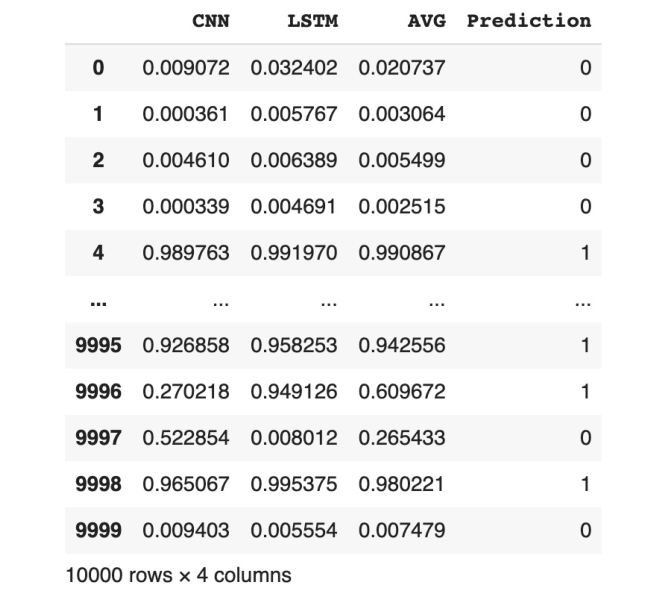
\includegraphics[width=0.55\linewidth]{images/chapter3/cnn-lstm.pdf}
	\caption{Wyniki połączenia modeli CNN i LSTM.}
	\label{fig:cnn-lstm}
\end{figure}


\noindent Zgodnie z naszą intuicją, osiągnęłyśmy pożądany efekt. Precyzja osiągnięta z tego połączenie wyniosła 90.98\%. Jest to najwyższy wynik wśród tych, które osiągnęłyśmy.

\begin{figure}[H]
	\centering
	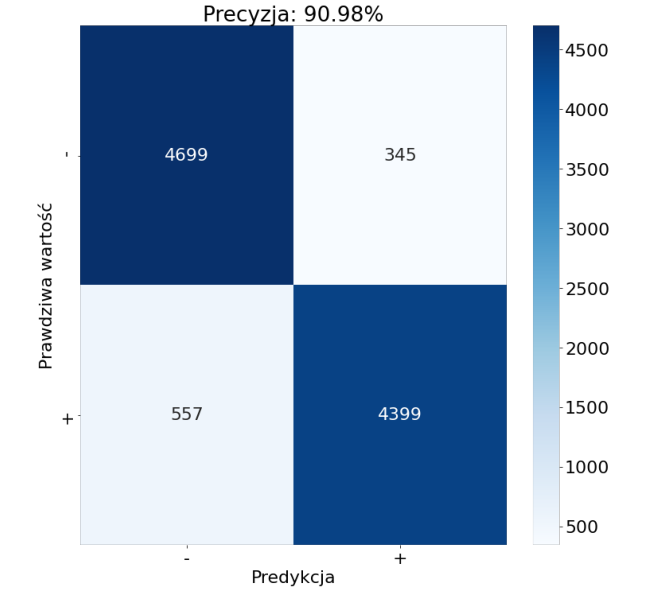
\includegraphics[width=0.55\linewidth]{images/chapter3/cnn-lstm-macierz.pdf}
	\caption{Macierz omyłek dla wyników z połączonych modeli CNN i LSTM.}
	\label{fig:cnn-lstm-macierz}
\end{figure}

\noindent Tradycyjnie kolorem granatowym zostały oznaczone wartości przewidziane prawidłowo przez skonstruowany przez nas model --- 4399 wartości zostały zaklasyfikowane prawidłowo jako pozytywne i 4699 wartości zostały zaklasyfikowane prawidłowo jako negatywne, co po zsumowaniu daje 9098 prawidłowo sklasyfikowane wartości na 10~000 przykładów. Tak więc precyzja predykcji wynosi 90.98\%. Ponadto 345 przykładów zostało błędnie sklasyfikowanych jako pozytywne i 557 błędnie jako negatywne. Został tu osiągnięty najlepszy wynik jeżeli chodzi o precyzję predykcji. Jednakże minus jest tu taki, że trzeba wytrenować zarówno sieć konwolucyjną jak i rekurencyjną, co sumarycznie zajmuje znacznie więcej czasu niż zajmowało to dla prostszych modeli, które dawały nie dużo gorsze wyniki. 

\section{Porównanie wyników dla wszystkich modeli}
W celu wyciągnięcia finalnych wniosków, porównałyśmy niektóre odpowiadające parametry stworzonych przez nas modeli. Te najważniejsze i decydujące zostały zestawione w poniższej tabeli (Tabela. \ref{tab:porównanie}). Modele posortowane zostały na podstawie precyzji --- od najmniej wydajnego do najbardziej wydajnego. 

\begin{table} [H]
	\caption{Porównanie czasów trenowania i precyzji wszystkich 5 modeli.}
	\label{tab:porównanie}
	\begin{center}
		\begin{tabular}{c | c c c c c c}
			\hline
			&  RF (D=32)      &  RF (D=64)  &       CNN         &     SVM         &    LSTM        &    CNN--LSTM \\
			\hline
			czas         &  4 min.       &   14 min.         &      22 min.     &     1 sek.        &    76 min.     &   22 + 76 min. \\
			precyzja  &  86.65\%       &    87.04\%     &    89.24\%     &     89.44\%    &   90.39\%     &     90.98\% \\
			\hline
		\end{tabular}  \\
		{\scriptsize 	RF --- Random Forest Classifier (maksymalna głębokość = 32 lub 64), SVM --- Support Vector Machine Classifier, CNN --- Convolutional Neural Network, LSTM --- Long Short-Term Memory\\}
	\end{center}
\end{table}

\noindent Nie zawsze bardziej skomplikowany model jest lepszy. W przypadku naszego zbioru danych oraz modeli widać, że różnice w precyzjach między skrajnymi modelami wynoszą tylko 4.33\%, natomiast czasy trenowania tych modeli znacznie się różnią. Pytaniem, które się tu nasuwa jest: jak by się wydłużyły te czasy gdybyśmy miały do czynienia z milionami przykładów trenujących? Należy się więc zawsze zastanowić, czy nie użyć prostszego modelu o nieco gorszej precyzji zyskując na czasie? \\
Godne uwagi jest działanie modelu klasyfikacyjnego wykorzystującego maszynę wektorów nośnych. Jak widać prosty liniowy model osiąglą precyzję równą aż 89.44\% (czyli jedynie 1.54\% gorszą od najlepszego modelu), przy czym całkowity czas trenowania wyniósł tylko 1 sekundę. Biorąc pod uwagę kompromis pomiędzy osiągniętą precyzją a czasem treningu, ten model uznałyśmy za najkorzystniejszy. \\


\begin{sidewaystable}
	\caption{Porównanie jednogłośności algorytmów.}
	\label{tab:porownanie-przyklady}
	\begin{tabular}{ |c|c|p{15cm}| c c c c c |}
		\hline
		nr rec.&	s &	rec.	&  	SVM &	RF &	CNN & LSTM & 	CNN--LSTM \\
		\hline
		35067& 0 & {\scriptsize I thought maybe... maybe this could be good. An early appearance by the Re-Animator (Jeffery Combs); many homage's to old horror movies; the Troma label on the front this movie could be a gem! I thought wrong.Frightmare is a boring, overplayed, half assed homage to the fright films of yore. The story is an old one, young people breaking into a house, getting drunk, making love, and tampering with things that shouldn't be tampered with. The oft recycled slasher film formula is used here, this time with a thought to be dead actor named Conrad Radzoff doing the killing. In fact, the performance by the Radzoff's actor Ferdy Mayne is the only redeeming quality of this film. He does the snooty Dracula style character very well. But as for the kids, its not so good, with Combs only having a minimal part.The film lacks entertainment value, and only features one cool character, and one or two scenes that can hold your attention. I do not recommend this film unless you are desperate for something to watch, and this is the only movie left at blockbuster.} &  0 & 0 & 0 &0 & 0 \\
		\hline
		
		12196 &		1 & {\scriptsize  Well, if you are one of those Katana's film-nuts (just like me) you sure will appreciate this metaphysical Katana swinging blood spitting samurai action flick.Starring Tadanobu Asano (Vital, Barren Illusion) \& Ryu Daisuke (Kagemusha). This samurai war between Heiki's clan versus Genji's clan touch the zenith in the final showdown at Gojo bridge. The body-count is countless.Demons, magic swords, Shinto priests versus Buddhist monks and the beautiful visions provided by maestro Sogo Ishii will do the rest.A good Japanese flick for a rainy summer night.} & 1 & 1 &1 &1&1 \\
		\hline
		49858&	1 & {\scriptsize  I liked this movie. That's pretty much all I can say about it. Lou Gossett did a good job, even though I'm still very disappointed in him after all the Iron Eagle movies. And even if I was smiling on the inside when the first main teenager dies (I won't give it away) it was done in a nice, fitting fashion. Pretty much everyone in this movie does a good job, so check it out! It's another one of those movies I found real cheap, so I bought it, and I recommend the same.} & 1&1&1&0&1\\	
		\hline
		46899 &		0&{\scriptsize  There is an inherent problem with commenting or reviewing a film such as this. I remember feeling the same way after disliking Dogma. If you do not like a film that is odd and controversial like Mulholland Dr., you are seen as "not getting it." Of course for those who have already seen this film you know that the entire point is not getting it anyway.I have heard from several different sources that the unique and likable aspect of this film is a dream-like quality it has. In other words, the plot isn't structured like other films. With the case of Mulholland Dr., it seems more like an unfocused collage made by a third grade boy who procrastinated until the last second to do his art project. It doesn't make sense, it isn't supposed to, but I know it was to be a TV series at first. It appears Lynch had a stack of unused film and decided to mash it in with a bunch of new stuff. You will notice that toward the end the nudity, sex and foul language increase. All things he would not have filmed for television.For a better film not told in a traditional, linear fashion, rent The Thin Red Line from 1998. That was a great film, this is not.Rating: 2 out of ten} & 0&0&1&1&1 \\
		\hline
	\end{tabular}
\end{sidewaystable}


\noindent Zauważyłyśmy również, że przypadku większości recenzji wszystkie modele rozstrzygały jednogłośnie o przynależności recenzji do danej klasy. Niemniej jednak, w przypadku niektórych recenzji różne modele różnie interpretowały ich wydźwięk i werdykt już nie był jednogłośny (Tabela. \ref{tab:porownanie-przyklady}). Powyżej znajdują się jedynie wybrane obrazujące to przykłady. Po analizie ustaliłysmy, że niezgodności występują w 138 przypadkach, gdzie prawidłowa wartość sentymentu była negatywna, a któryś z algorytmów przewidział wartość pozytywną, a odwrotna sytuacja miała miejsce w 99 przypadkach. \\

\bigskip
\noindent Inspirację do stworzenia modeli opartych o sieci neuronowe zaczerpnęłyśmy z publikacji \cite{minaee2019deep}, dlatego też osiągnięte przez nas wyniki dla odpowadających modeli porównałysmy z tymi, które otrzymali autorzy publikacji. Należy tutaj wspomnieć, że wykorzystali oni nieco inne warunki trenowania i testowania, a mianowicie podzielili wyjściowy zbiór w inny sposób --- 50\% recenzji użyli do trenowania a kolejne 50\% do wykonania testów. U nas natomiast trening odbywał sie na 80\% przykładów a testy obejmowały 20\%.

\begin{table} [H]
	\caption{Wyniki naszego modelowania vs. wyniki opublikowane przez Minaee et al. \cite{minaee2019deep}.  Parametrem porównywanym jest precyzja.}
	\begin{center}
		\begin{tabular}{c |c|c }
			\hline
			Model &  Nasze wyniki   &  Wyniki Minaee et al. \\
			\hline
			CNN & 89.24\% & 89.3\% \\ 
			LSTM & 90.39\% & 89\% \\ 
			CNN--LSTM &90.98\% & 90\%\\ 
			\hline
		\end{tabular}
	\end{center}
\end{table}

\noindent Jak widać udało nam się odtworzyć wyniki z przedmiotowej publikacji. Osiągnęłysmy wyniki porównywalne dla modelu CNN, a dla pozostałych dwóch nawet nieco lepsze niż autorzy. Jednak, tak jak wspominałyśmy, Minaee et al. mieli mniej przykładów żeby sie dobrze nauczyć a zarazem wiecej przykładów, w których ich modele miały szanse się pomylić. Osiągnięte przez nas różnice są de facto znikome, więc finalnie można ogłosić remis.